\section{L'analyse d'image et ses formes}
\label{conv_sec}
\subsection{Les différentes thématiques de l'analyse d'image}
L'analyse d'image est un domaine d'application vaste et dont la recherche est très active. Les applications industrielles sont très riches et très diversifiées telles que l'imagerie médicale, l'automatisation des transports (véhicules autonomes) ou encore la robotique. \\

\noindent Les principales thématiques de l'analyse d'image\footnote{Les noms des thématiques sont relativement flous et inconstants dans la littérature. Il est possible que certaines personnes en utilisent d'autres voire associent des noms à un autre problème. Retenez le contexte des problèmes plutôt que les noms !} sont:
\begin{itemize}
    \item \textbf{Classification}: Cette thématique est la plus classique. L'objectif est de catégoriser les images selon l'entité qu'elle représente. La classification est non-absolue, i.e l'image est catégorisée comme positive à une classe si une entité caractérisant cette classe est représentée. Néanmoins, d'autres entités peuvent être représentées sur cette image aussi. Par exemple, une image représentant une voiture en ville peut être labellisée "voiture" malgré la présence d'autres entités comme un autre type de véhicule, une personne etc... Généralement, le label définissant l'image est le label défini comme le plus probable. Néanmoins, il est possible d'assouplir cette limitation en ne considérant pas la classe la plus fiable mais les différentes classes dont la prédiction est supérieure à une valeur seuil. Cette tâche est la plus basique et la plus exploitée aujourd'hui. Le prestige des compétitions de classification sont comparables au 100m en athlétisme et constitue la vitrine de l'analyse d'image. En effet, elle mettent en avant les innovations d'architectures neuronales et pose les fondations des évolutions permanentes qui alimenteront par la suite, les autres problématiques. Les réseaux décrites dans la Section \ref{convsecmain} sont les solutions State-of-the-art.

    \item \textbf{Object Detection}: Cette thématique cherche à localiser spatialement une classe d'entité sur une image. L'objectif est donc de délimiter une sous-partie de l'image représentant la classe à détecter. Ce type d'analyse est binaire, i.e une surface peut être classée comme positive ou négative. Il n'y a donc qu'un type d'entité détectable possible. La surface classée positivement est souvent délimitée par un rectangle. L'un des problèmes les plus étudiés correspond à la reconnaissance faciale (\textit{Face Recognition}).

    \item \textbf{Object Recognition}: Cette thématique généralise \textit{Object detection}. Elle cherche à détecter de multiples entités correspondant à différentes classes dans une image et à déterminer leurs localisations. Cette méthode est très utilisée par les outils de mesure et de surveillance notamment par les drones et les caméras de surveillance.

    \item \textbf{Object Tracking}: Cette problématique est associée aux contraintes de mouvements et de temps réel. L'objectif est de repérer une (des) entité(s) et de réaliser un suivi en temps réel en gardant l'attention sur ces objets. Cette problématique est associée au support vidéo et peut être vue comme une généralisation de \textit{Object recognition} avec une contrainte de temps-réel. Néanmoins, la considération de la dimension temporelle soulève plusieurs difficultés notamment la définition d'un phénomène temporel défini sur plusieurs images successives ou la variation d'une entité à suivre comme un individu qui porte puis enlève un chapeau. La classification de l'entité n'est pas impératif. Sous contraintes de vélocité, de nombreux algorithmes de \textit{Tracking} néglige la classification. En effet, la présence du phénomène de \textit{tracking} est associée à la présence d'une entité "de valeur"\footnote{On ne sait pas de quelle classe est l'entité précisément mais on sait que c'est une entité d'importance.}, ce qui est une information souvent suffisante à l'exploitation métier. Le \textit{Tracking} se découpe en deux problématiques principales qui sont le \textit{Tracking} mono-cible et le \textit{Tracking} multi-cible.

    \item \textbf{Semantic Segmentation}: Cette approche cherche à analyser une image au niveau du pixel. C'est-à-dire qu'elle cherche à assigner un pixel à une classe. La discrimination spatiale des entités sur l'image est ainsi bien plus importante. Néanmoins, la différenciation se fait au niveau sémantique et non des instances, de ce fait, seulement une différenciation de classe est réalisée et non des entités-même\footnote{Supposons une foule d'individus dense, Semantic segmentation ne sera pas capable de différencier chacun des individus et généralisera à une surface globale classifiée comme "individu".}.

    \item \textbf{Instance Segmentation}: Cette approche est similaire à \textit{Semantic segmentation} mais la discrimination se fait au niveau des entités et non des classes. Ainsi, en reprenant l'exemple d'une foule, l'objectif de \textit{Instance segmentation} est de discriminer l'ensemble des individus de manière unitaire et non un ensemble correspondant à une classe "individus". Cette méthode est très utilisée en imagerie médicale notamment dans l'analyse de cellules cancéreuses.

    \item \textbf{Object Proposal}: Cette approche correspond à une analyse exploratoire. Elle cherche à isoler des sous-parties d'une image susceptible de contenir une entité de valeur.

    \item \textbf{Text Detection}: Cette thématique est associée à la détection de texte dans une image. Elle a pour objectif de détecter, localiser et extraire les entités textuelles présentes sur une image. Cette problématique est souvent associée à la transcription d'un texte manuscrit (en photo) ou de fichiers non éditables caractérisant un texte tels qu'un scan sous un format d'image (.jpeg ou .png par exemple). Une thématique connexe (\textit{Handwriting recognition}) est souvent associée et consiste à unir un texte à un auteur selon les spécificités du style d'écriture\footnote{Cette approche se base quasi-exclusivement sur l'analyse du style graphique d'écriture. Le style syntaxique n'est pas traité.}.

    \item \textbf{Landmark Detection}: Cette problématique correspond à la détermination de la position d'un point de référence d'une entité et de son orientation par rapport à un système de coordonnée (par exemple, l'étude de points spécifiques déterminant la posture d'un individu (\textit{Pose Estimation}). Cette problématique est très utilisée par les systèmes autonomes afin d'avoir une meilleure compréhension de son environnement local et des intéractions à réaliser. L'exemple populaire de ce type d'outils sont les filtres de photo/vidéo d'applications mobiles telles que Snapchat ou Instagram.

    \item \textbf{Image Captionning}: Cette problématique est associée à la génération d'une description textuelle d'une image. Elle unit l'analyse d'image (Computer Vision) et le Traitement du langage naturel (Natural Language Processing).
\end{itemize}

\noindent Un exemple illustratif de ces différents problèmes est visible sur la Figure \ref{classifim}.

\begin{figure}
    \begin{tabular}{cc}
    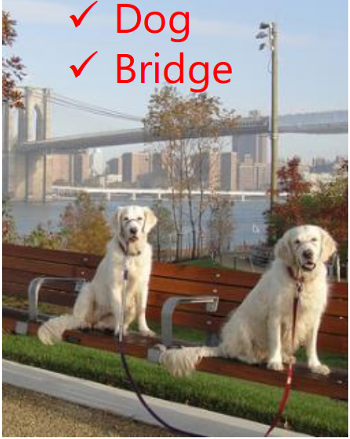
\includegraphics[scale=0.25]{./tex/computer-vision/object-recognition/classifim.png}&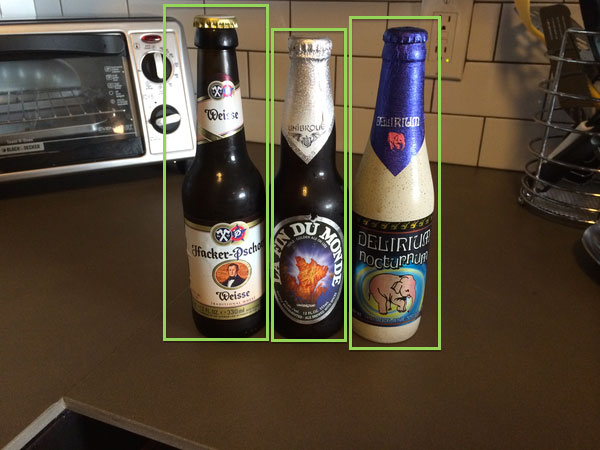
\includegraphics[scale=0.2]{./tex/computer-vision/object-recognition/detecobj.jpg}\\
    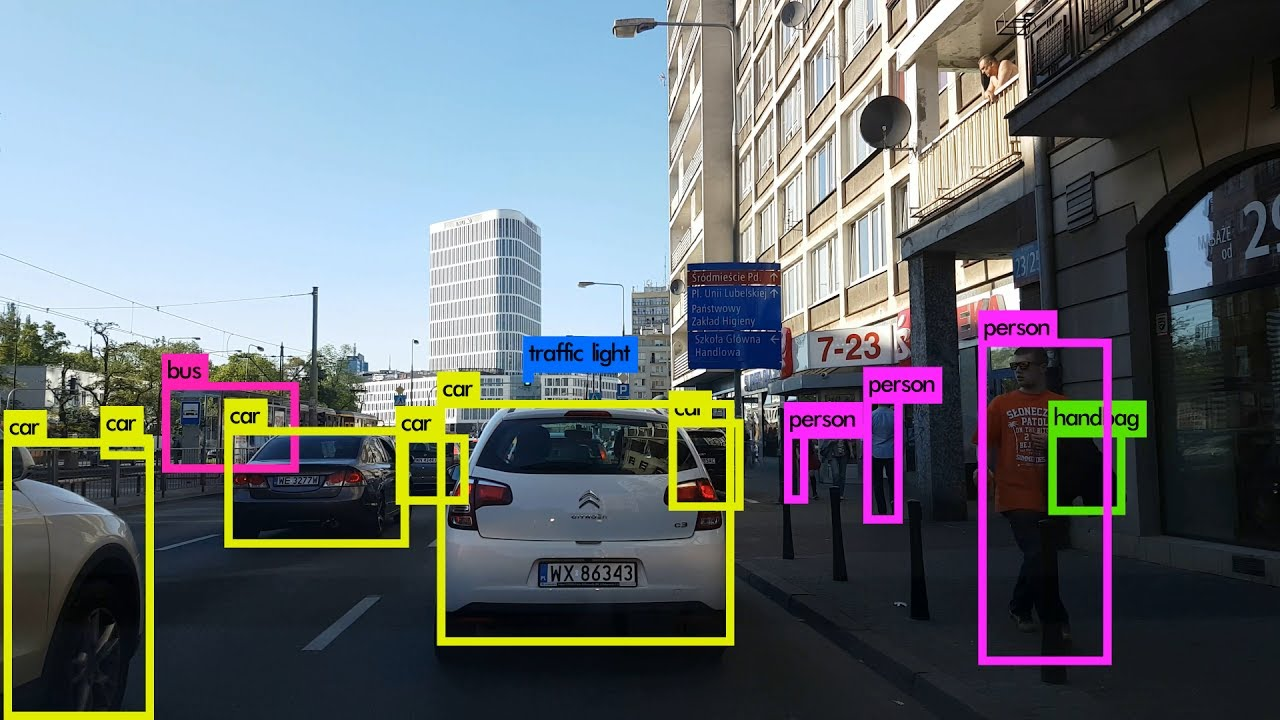
\includegraphics[scale=0.11]{./tex/computer-vision/object-recognition/recodetec.jpg}&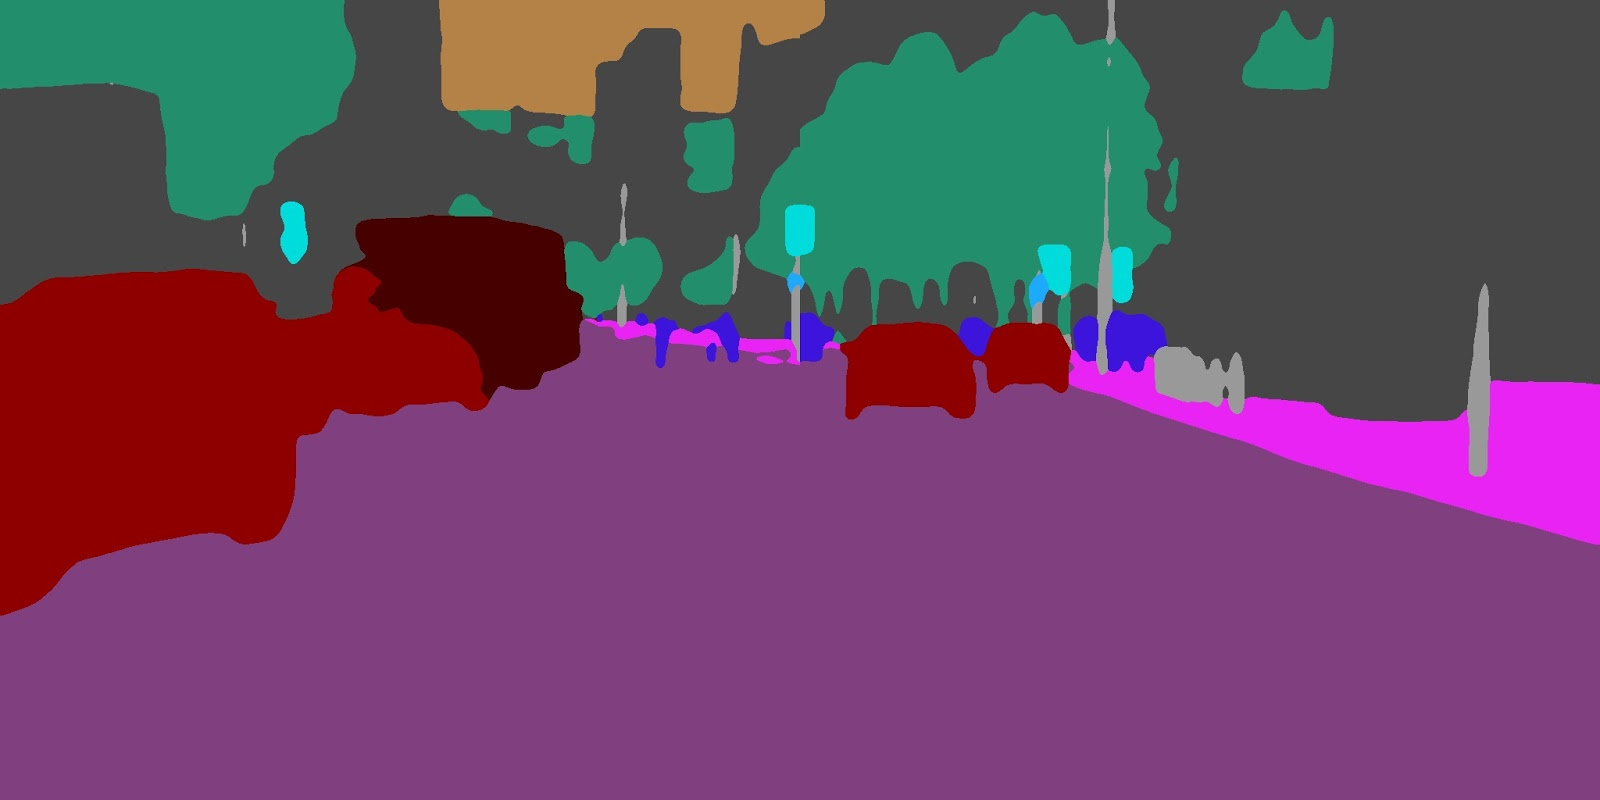
\includegraphics[scale=0.1]{./tex/computer-vision/object-recognition/segsem.jpg}\\
    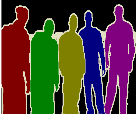
\includegraphics[scale=0.8]{./tex/computer-vision/object-recognition/instanceseg.png}&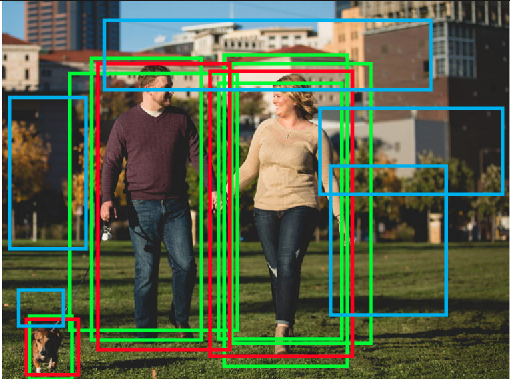
\includegraphics[scale=0.25]{./tex/computer-vision/object-recognition/objprop.png}\\
    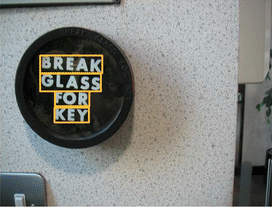
\includegraphics[scale=0.4]{./tex/computer-vision/object-recognition/textdetepic.png}&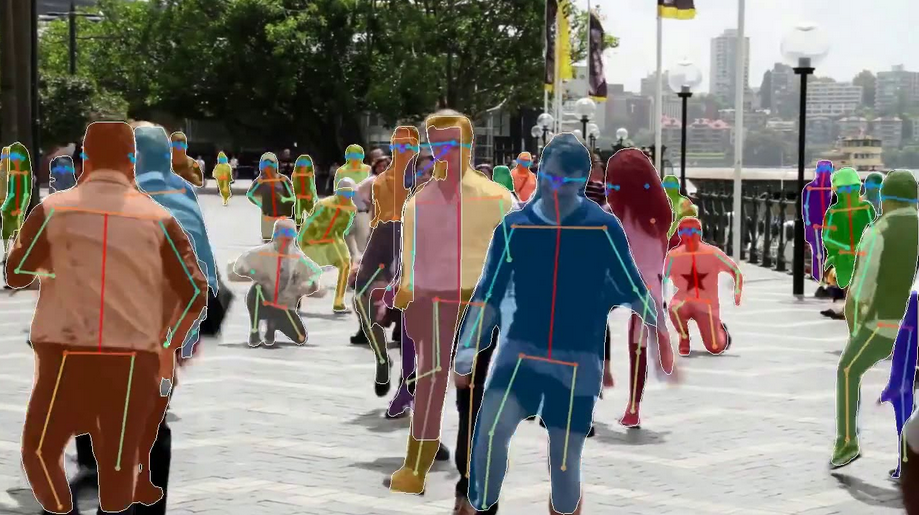
\includegraphics[scale=0.2]{./tex/computer-vision/object-recognition/poseest.png}\\
    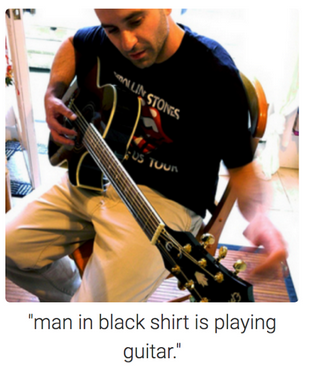
\includegraphics[scale=0.4]{./tex/computer-vision/object-recognition/imagecappic.png}
    \end{tabular}
    \caption{Exemple d'analyse d'image: 1) Classification, 2) Object detection, 3) Object recognition, 4) Segmantic segmentation, 5) Instance segmentation, 6) Object proposal, 7) Text Detection, 8) landmark Detection (Pose estimation), 9) Image Captionning}
    \label{classifim}
\end{figure}

\subsection{Généralités théoriques}
\subsubsection{Théorie - Object Detection, un problème de Régression}
Supposons une problématique d'\textit{Object Detection}. L'objectif est donc de détecter la classe d'une image et de localiser l'entité de valeur sur l'image. Pour isoler l'entité de valeur, nous chercherons à réaliser un rectangle qui délimitera sa surface.\\

\noindent Un rectangle peut être défini de plusieurs manières\footnote{La manière de représenter le rectangle est déterminée par la méthode employée dans le jeu d'apprentissage. Cette méthode doit être identique pour toutes les données !}. Dans notre configuration, nous définirons un point qui déterminera le centre ($b_x$,$b_y$) de l'entité de valeur et ($b_h$,$b_l$), hauteur et largeur du rectangle. Une illustration est visible sur la Figure \ref{objdetec}.\\

\noindent L'objectif du réseau prédictif est donc de prédire une classe d'image et 4 coordonnées spatiales ($b_x$,$b_y$,$b_h$,$b_l$). Supposons un réseau qui doit discriminer 3 classes: (1) chien, (2) chat, (3) voiture. La première problématique est de définir la structure de la sortie du réseau (et donc du label des données). Pour rappel, il est nécessaire d'avoir les différentes coordonnées du rectangle délimiteur (bounding boxe) et le label de la classe d'image sachant qu'une image peut ne pas représenter une classe d'objet. Une représentation peut donc être:\\

\noindent Soit y, la sortie du réseau prédictif tel que: $$y=[p_c,b_x,b_y,b_h,b_l,c_1,c_2,c_3]$$
\begin{itemize}
    \item $p_c$: valeur binaire - Si une classe est représentée, $p_c$=1 sinon 0.
    \item $b_x,b_y,b_h,b_l$: valeur numérique - Coordonnées du rectangle délimiteur où $b_x,b_y$, coordonnées du point central de l'entité.
    \item $c_1,c_2,c_3$: valeur binaire - Si la classe i est représentée, $c_i$=1 sinon 0. Seule une classe peut être représentée sur une image.
\end{itemize}

\noindent Supposons une image représentant un chien, alors la sortie du réseau prédictif sera de la forme: $$y=[1,b_x,b_y,b_h,b_l,1,0,0]$$
\noindent De même, supposons une image ne représentant aucun classe, nous obtiendrons:
$$y=[0,b_x,b_y,b_h,b_l,0,0,0]$$

\noindent Il est \textbf{important} de savoir que dans le cas d'une image non classée, le contenu du vecteur de sortie ne présente \textbf{aucune importance} en terme de valeurs exceptée la valeur de $p_c$. Les valeurs du réseau peuvent donc être arbitraires, de même que celles du vecteur référence pour l'apprentissage.\\

\noindent Il reste à définir une fonction de coût. Observons que nous avons 3 types de problématiques: le problème bi-classe ($p_c$), le problème de régression ($b_x,b_y,b_h,b_l$) et le problème multi-classe ($c_1,c_2,c_3$). Il est donc nécessaire d'utiliser une fonction de coût qui soit capable de considérer ces trois problèmes. De même, elle doit être capable de considérer la particularité de l'absence de classe sur une image.\\

\noindent Définissons y comme le label d'apprentissage et y', label prédit. Une solution peut être définie par:\\

\noindent Si $y_{p_c}$ = 1:
$$\mathcal{L}(y,y')=\mathcal{L}_{binary}(p_c,p_c')+\mathcal{L}_{regression}(\sum b, \sum b')+\mathcal{L}_{Nclasse}(\sum c, \sum c')$$
\noindent Si $y_{p_c}$ = 0:
$$\mathcal{L}(y,y')=\mathcal{L}_{binary}(p_c,p_c')$$

\noindent $\mathcal{L}_{binary}$ doit être capable de mesurer l'erreur d'un problème binaire. \textit{Cross entropy loss} est donc une possibilité. Pour $\mathcal{L}_{regression}$, \textit{Mean Squared error} est une possibilité et pour $\mathcal{L}_{Nclasse}$, \textit{Negative Logarithmic Likelihood}\footnote{Il ne faut pas oublier le danger du log(0) !}. Il est possible d'utiliser d'autres fonctions tant qu'elles respectent les particularités de chaque problématique.

\begin{figure}
    \centering
    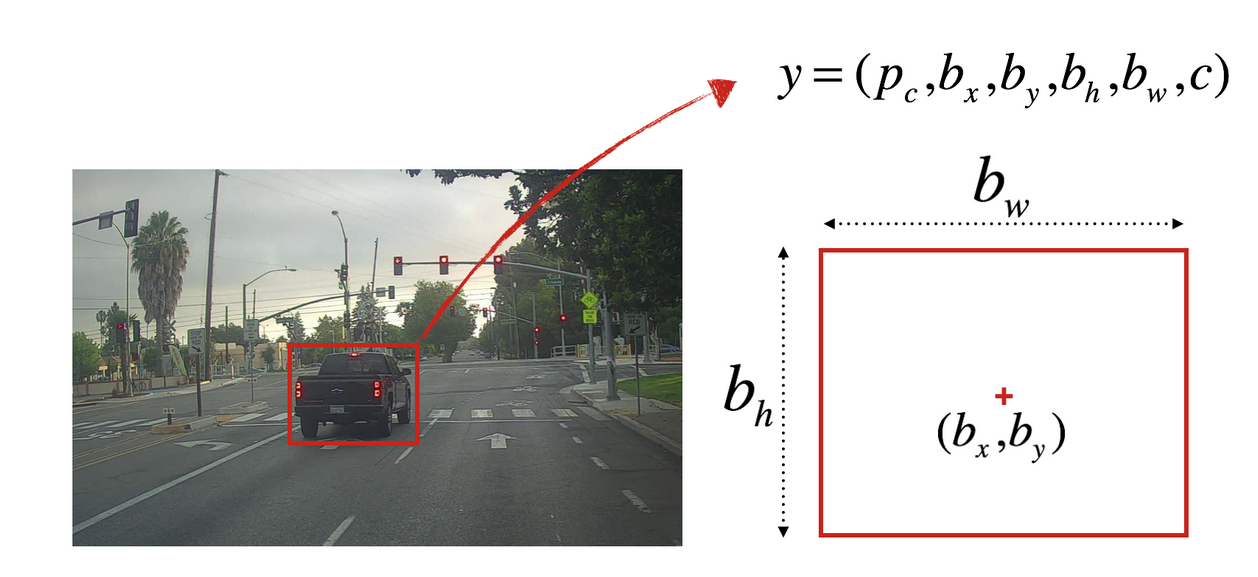
\includegraphics[scale=0.3]{./tex/computer-vision/object-recognition/detepi.png}
    \caption{Exemple - Object Detection}
    \label{objdetec}
\end{figure}

\subsubsection{Théorie - Landmark detection, un problème de Régression}
Cette approche est similaire à une généralisation de l'\textit{Object Detection}. Supposons un problème de détection de points de références pour une analyse de visage par exemple. Ces points peuvent déterminer la position des yeux, des lèvres etc... Un exemple est visible sur la Figure \ref{landmarkdec}.\\

\noindent Au lieu de déterminer un rectangle, cette problématique cherche à déterminer la localisation de différents points soit des couples de la forme ($pr_x,pr_y$). Ainsi, supposons la présence de 128 points de références, il faudra donc 128 couples ($pr_x,pr_y$) soit 256 valeurs. Il est important de considérer la possibilité de présence ou non de la classe qu'on cherche à déterminer. On supposera un système qui reconnaît qu'une classe spécifique. Il faudra donc une variable binaire comme vu dans la section précédente. Ainsi, le vecteur de prédiction sera de la forme:
$$y=[p_{classe}, \sum_{128} (pr_{x,i},pr_{y,i})]$$

\begin{figure}
    \centering
    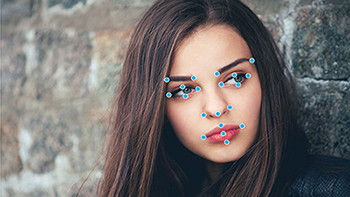
\includegraphics[scale=1.3]{./tex/computer-vision/object-recognition/landmark.jpg}
    \caption{Exemple - Landmark Detection}
    \label{landmarkdec}
\end{figure}

\subsubsection{Sliding Windows}
\textit{Object Recognition} se distingue de \textit{Object Detection} par le nombre d'entités détectables sur une image. En autorisant la détection d'un nombre indéterminé d'entités, la dimension de sortie des réseaux neuronaux n'est plus déterminable à l'avance. Il est donc nécessaire de proposer une approche qui permet de résoudre des problèmes de multi-détection en se ramenant à un problème mono-détection. Une solution (historique) s'appelle \textit{Sliding Windows}.\\

\noindent Supposons une image $I_{raw}$ de dimension N*N. L'algorithme du \textit{Sliding Windows} consiste à définir une \textit{fenêtre} (window) de dimension M*M telle que $M \leq N$ qui isolera une sous-partie de l'image initiale que nous appellerons $I_{crop,i,j}$ avec i,j coordonnées du point de référence\footnote{On peut associer un point de référence à un pixel de la matrice d'image} de $I_{raw}$. Nous supposerons que ce point de référence est indiqué par le coin supérieure gauche de la fenêtre. Dans notre exemple, il y a N*N points de référence. Nous souhaitons que notre fenêtre soit intègre, i.e qu'elle soit contenu dans l'image initiale. Il y a donc (N-M+1)*(N-M+1) position possible pour notre fenêtre. Ainsi, nous faisons \textit{glisser} notre fenêtre sur les (N-M+1)*(N-M+1) positions possibles. Une illustration est visible sur la Figure \ref{slidewind}.\\

\noindent Nous obtenons ainsi un ensemble d'images caractérisant l'image initiale. Chacune des images est analysée par un réseau prédictif (convolutif) et une classification est réalisée. Le réseau prédictif doit déjà être entrainé sur la tâche à réaliser et peut être binaire (classification mono-classe) ou multi-classe.\\

\noindent Ce cycle est réalisé avec différentes dimensions de fenêtre (grande et petite) afin de réaliser une discrimination efficace de l'image. De même, le pas de glissement de la fenêtre peut être différente qu'unitaire afin de balayer plus grossièrement l'image à traiter. Une particularité est \textbf{importante}. Du fait de la variation de la dimension de la fenêtre, la dimension de l'image à analyser par le réseau diffère. Un réseau de neurones peut traiter une donnée avec une dimension fixe uniquement. Il est donc important de s'assurer que le réseau reçoit une donnée de dimension unique. Deux méthodes sont possibles: exploiter autant de réseaux distincts qu'il y a de dimension possible aux fenêtres. Cette méthode est sans doute la plus efficace mais particulièrement gourmande en temps d'apprentissage. La seconde approche est de réaliser un redimensionnement de l'image avec des méthodes de \textit{Downsampling} ou \textit{Upsampling}.\\

\noindent Dans les faits, cette méthode n'est pas exploitable avec des approches neuronales du fait du temps calculs bien trop élevé. Le nombre d'étape \textit{Forward} est bien trop important à cause de la quantité d'images obtenues par le fenêtrage. Cette méthode est, cependant, encore employée avec des outils de classification plus rudimentaires et donc rapides mais la qualité de la prédiction est diminuée. Malgré tout, l'idée du \textit{Sliding Windows} est encore au coeur des algorithmes à l'état de l'art. Seule son implémentation diffère afin de le rendre exploitable avec des approches neuronales. De plus, \textit{Sliding Windows} présente un problème majeur: la position de ses fenêtres. En effet, les fenêtres sont de tailles fixes et le déplacement de la fenêtre est fixé. Il est donc probable que de nombreuses entités ne puissent être parfaitement localisées. Un exemple de cette limitation est visible sur la Figure \ref{slidewindconvyl}. Ce type d'approche est donc peu efficace en cas d'entités aux dimensions variables. Il est, cependant, possible d'exploiter l'algorithme du \textit{Sliding Windows} avec différentes dimensions de fenêtre mais le coût en calcul devient rapidement trop important du fait de la multitude de dimension nécessaire pour envisager une détection viable.

\begin{figure}
    \centering
    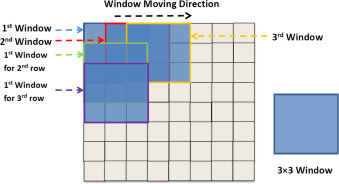
\includegraphics[scale=1]{./tex/computer-vision/object-recognition/slidewin.jpg}
    \caption{Exemple - Sliding Windows}
    \label{slidewind}
\end{figure}

\begin{figure}
    \centering
    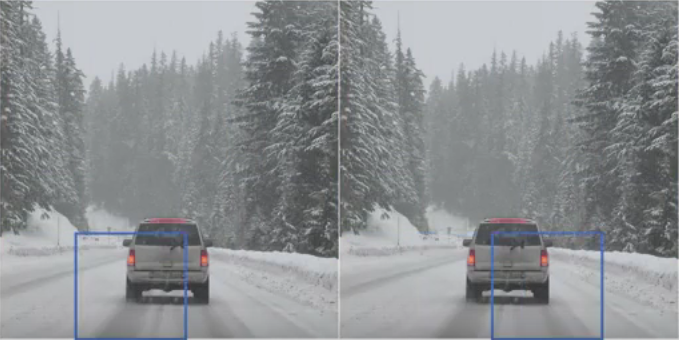
\includegraphics[scale=0.4]{./tex/computer-vision/object-recognition/yl1.png}
    \caption{Limitation du Sliding Windows}
    \label{slidewindconvyl}
\end{figure}

\subsubsection{Sliding Windows et réseau convolutif}
Dans la Section \ref{convfctoconv}, nous avons vu comment convertir une couche Full-Connected en couche de convolution. La méthode \textit{Sliding Windows} est trop gourmande en temps machine comme vu dans la Section précédente. Une implémentation intégralement convolutive est possible pour limiter le coût de calcul de cet algorithme.\\

\noindent Observons la Figure \ref{slidewindconv}. Le réseau du haut présente un réseau convolutif standard. L'image d'entrée est de 14*14 (on négligera la profondeur pour l'exemple) et la sortie 1*1. L'intégralité de l'information portée par l'image d'entrée est donc résumée par la sortie de ce réseau.\\

\noindent Supposons maintenant une image de dimension plus grande (16*16). En gardant la même configuration de réseau que celui décrit précédemment, on observe une sortie de la forme 2*2. Du fait du comportement de fenêtre glissante des couches de convolutions, l'action de \textit{Sliding Windows} est réalisée par le calcul-même des convolutions. Observons le rectangle rouge de la donnée d'entrée, il correspond à une matrice 14*14 (similaire à la matrice d'entrée de l'autre réseau). Nous observons au fil du réseau que l'information portée par cette surface de la matrice est expliquée par le carré supérieure droit de la sortie. En prenant l'exemple du rectangle mauve, il va s'agir du carré inférieure gauche. Nous pouvons donc constater que ce réseau est similaire à l'action du \textit{Sliding Windows} pour une fenêtre carrée de taille 14 et de stride 2 (réalisée par l'étape du Pooling). Cependant, il n'a réalisé qu'une étape Forward pour réaliser ces prédictions. Un gain de temps majeur est donc réalisé en limitant la redondance de calculs.

\begin{figure}
    \centering
    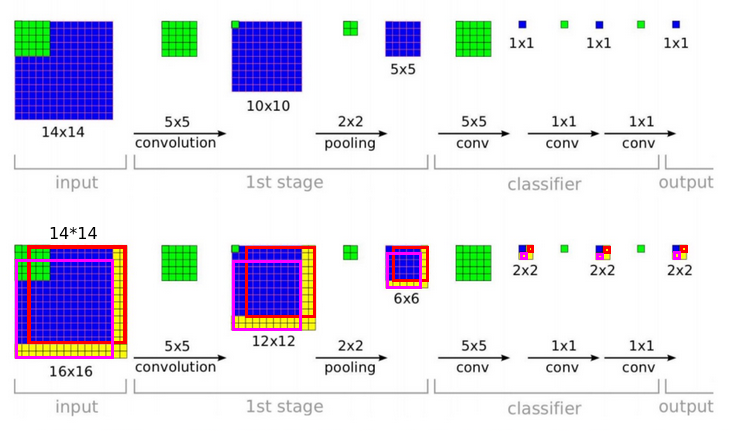
\includegraphics[scale=0.4]{./tex/computer-vision/object-recognition/convwd.png}
    \caption{Exemple - Convolutive Sliding Windows}
    \label{slidewindconv}
\end{figure}

\subsubsection{Region Proposal}
Au lieu de se limiter à l'optimisation de calcul du \textit{Sliding Windows}, une approche visant à optimiser le nombre de fenêtres (de dimension \textbf{non fixe}) à analyser serait intéressante. Cette approche est exploitée par les algorithmes \textit{Region Proposal}.\\

\noindent L'objectif de ces algorithmes est de déterminer des régions d'intérêts sur une image, i.e déterminer des \textit{bounding boxes} susceptibles de contenir une entité. Il est \textbf{important} de comprendre que ces algorithmes ne réalisent pas de classification. Ils isolent des parties de l'image qui pourraient contenir une entité sans analyser la nature de l'entité isolée. La condition principale de ces algorithmes est d'avoir un grand \textit{Rappel}. En effet, il est possible de filtrer des faux positifs avec les algorithmes de classification. Par contre, si une entité n'est pas isolée par une \textit{bounding boxe}, elle ne pourra \textit{jamais} être détecter par l'algorithme d'\textit{Object Detection}. Il est donc nécessaire de ne pas être trop sévère sur la création des fenêtres. Ainsi, les \textit{bounding boxes} crées peuvent être bruitées, se superposer mais il est probable que l'une d'elles isolent l'entité de manière satisfaisante.\\

\noindent \textit{Region Proposal} repose sur la notion de \textbf{segmentation} d'image. La \textit{segmentation} permet de grouper différentes régions de l'image selon des critères de similarité tels que l'analyse de couleur, de texture\footnote{Ces analyses relèvent de l'analyse d'image traditionnelle. Elles ne seront pas approfondies dans ce cours}... Ces régions unies discriminent des surfaces d'intérêts et permettent de définir des \textit{bounding boxes} de dimension variables et spécifiques à ces zones d'intérêts tout en étant moins nombreuses qu'une recherche exhaustive comme réalisée par \textit{Sliding Windows}.\\

\noindent Il existe différents algorithmes de \textit{Region Proposal}. Le plus populaire et utilisé est \textbf{Selective Search}, notamment du fait d'être la méthode employée par des méthodes d'\textit{Object Detection} parmi les plus performantes\footnote{Ces méthodes tendent à devenir obsolètes avec les dernières avancées} (R-CNN et Fast R-CNN).

\paragraph{Selective Search}

\textit{Selective Search} est un algorithme de \textit{Region Proposal} dans le cadre de la détection d'objet. Son objectif est d'avoir un fort \textit{Rappel} et d'être rapide. La segmentation de l'image est réalisée par une méthode \textit{graph-based} développée par Felzenszwalb and Huttenlocher\cite{segss}\footnote{Nous ne détaillerons pas cette méthode. Il faut juste retenir que c'est une technique de segmentation d'image. Vous pouvez lire l'article de recherche indiqué si vous souhaitez approfondir son étude.}. Un exemple d'application de cette méthode est visible sur la Figure \ref{segssim}.\\

\noindent \textit{Selective Search} exploite une image segmentée et réalise une procédure itérative en deux étapes:
\begin{itemize}
    \item Création des \textit{bounding boxes} correspondant aux différentes surfaces segmentées
    \item Union des surfaces segmentées qui présentent une similarité élevée
\end{itemize}

\noindent Cette procédure est répétée jusqu'à ce que l'image segmentée ne soit plus modifiée par l'étape d'union ou que l'image présente une unique catégorie. Un exemple est visible sur la Figure \ref{selese}.\\

\noindent La mesure de similarité de \textit{Selective Search} est une combinaison linéaire de 4 autres métriques sous-jacentes: similarité par couleur, par taille, par texture et par forme. Nous ne détaillerons pas ces métriques, veuillez vous référer à l'article associé.

\begin{figure}
    \centering
    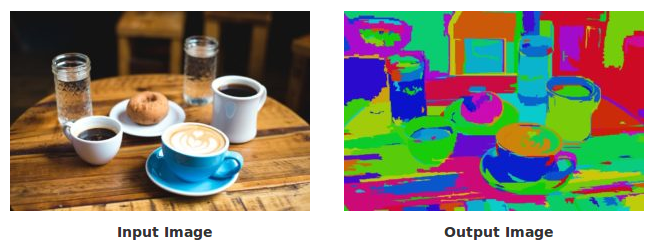
\includegraphics[scale=0.4]{./tex/computer-vision/object-recognition/segss.png}
    \caption{Exemple - Graph-based Segmentation}
    \label{segssim}
\end{figure}

\begin{figure}
    \centering
    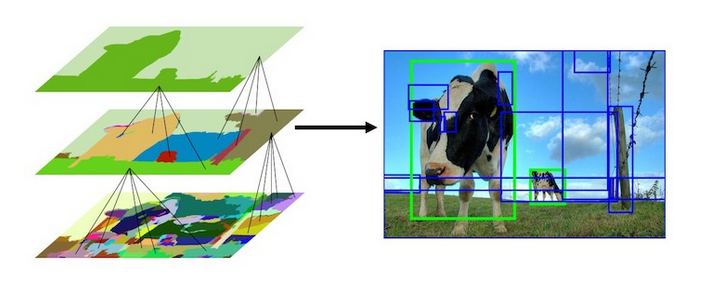
\includegraphics[scale=0.4]{./tex/computer-vision/object-recognition/ssim2.png}
    La suppression des bounding boxes doublons ou inexactes n'est pas réalisée par Selective Search
    \caption{Exemple - Selective Search}
    \label{selese}
\end{figure}

\subsubsection{Anchor Boxes}

Bien qu'efficace, \textit{Selective Search} est un point faible de plusieurs algorithmes de l'état de l'art. Plus lent que l'étape Forward d'un réseau convolutif, il est le facteur limitant à la vélocité des systèmes actuels (R-CNN et Fast R-CNN). Une solution alternative a été crée: \textbf{Anchor boxes}.\\

\noindent \textbf{Anchor Boxes} définit des fenêtres prédifinies avec des tailles différentes (64*64, 128*128 par exemple) et des ratios différents (1:1, 2:1, 1:2 par exemple) centrées en un même centre. Une illustration est visible sur la Figure \ref{anchor}.\\

\noindent Supposons l'image d'entrée comme une surface quadrillée selon chaque pixel. Une image 200*200 serait donc équivalent à un quadrillage 200*200. Nous définissons nos \textit{anchors} selon l'exemple décrit sur la Figure \ref{anchor}. Il y a donc 9 \textit{anchors} distincts. Un centre d'\textit{anchors} est positionné sur chaque case du quadrillage. Il y aura donc 200*200*9=360 000 \textit{anchors} distincts. Dans les faits, il n'est pas nécessaire d'imposer une aussi grande sensibilité\footnote{Un pixel ne "sépare" pas deux entités distinctes en général...}. Il est donc possible d'appliquer un stride sur le positionnement des centres. Par exemple, supposons un stride de 20. Il y aura donc 11*11 centres soit 1089 \textit{anchors} distincts. Bien que ce nombre puisse impressionner, il est faible (ou équivalent selon le cas) comparé aux nombre de fenêtres obtenues par \textit{Sliding Windows} et \textit{Region Proposal}. Grossièrement, nous pouvons donc dire que \textit{Anchor Boxes} réalise le même travail (détermination de \textit{bounding boxes}) que \textit{Region Proposal} excepté qu'il produit des \textit{bounding boxes} de dimensions prévues à l'avance. Ce type d'approche est efficace car il est plus facile d'adapter les dimensions d'une fenêtre que de les prédire intégralement. Ainsi, on peut créer des \textit{anchors} dont la forme est grossièrement adaptée à la forme de l'entité à observer - par exemple, une fenêtre haute et peu large pour un individu - et le réseau s'occupera d'affiner les dimensions pour coller au mieux à l'objet observé.

\begin{figure}
    \centering
    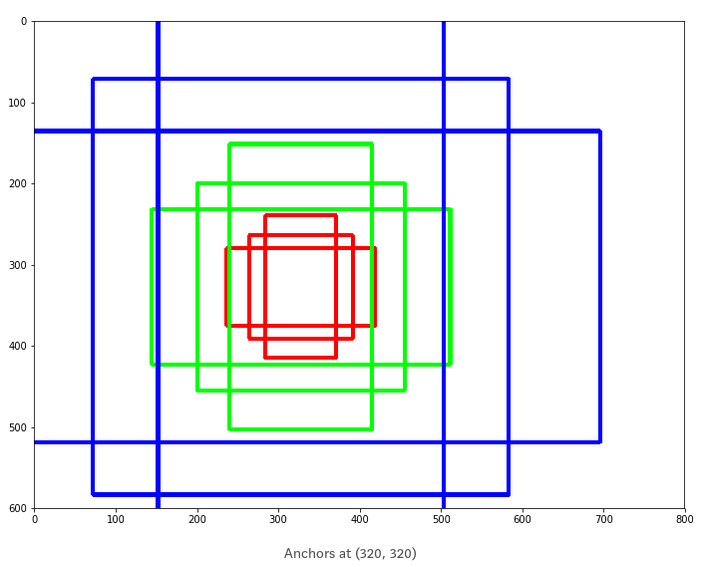
\includegraphics[scale=0.3]{./tex/computer-vision/object-recognition/anchor.png}
    \\3 tailles: 128x128, 256x256, 512x512\\
    3 ratios: 1:1, 1:2, 2:1
    \caption{Exemple - Anchor Boxes}
    \label{anchor}
\end{figure}


\subsubsection{RoI Pooling}

La création de \textit{bounding boxes} soulève une problématique importante: la dimension variable des fenêtres. Cet aspect est critique car un réseau neuronal ne peut accepter qu'une entrée à valeur fixe. Il est donc important de proposer une méthode d'uniformisation des dimensions des \textit{bounding boxes}. \\

\noindent Une autre condition d'optimisation est caractéristique de cette méthode. En effet, il est tout à fait envisageable d'extraire chaque sous-partie d'une image discriminée par une \textit{bounding boxes} et de réaliser un redimensionnement (cropping, warping...). Bien que parfaitement fonctionnelle, si on suppose qu'il y a 1000 \textit{bounding boxes} crées, cette technique va imposer 1000 étapes Forward aux couches de convolution suivantes pour extraire les attributs de l'image\footnote{Sous-partie de l'image de départ délimitée par une \textit{bounding boxes}} analysée. En effet, avec cette approche, on considère une sous-partie de l'image d'origine, pas une \textit{feature map} issues d'un réseau convolutif qui a traité cette image. Ceci est très coûteux en temps de calcul. En effet, il est probable que de nombreuses \textit{bounding boxes} se chevauchent. Calculer leurs sorties d'un réseau convolutif reviendrait à réaliser de la redondance calculatoire en réalisant les mêmes calculs plusieurs fois sur une même surface de la matrice de l'image d'origine. \textit{RoI Pooling} propose une approche qui permet de s'émanciper de l'image initiale brute et d'exploiter les \textit{feature map} qui lui sont associées uniquement. Cette particularité est très importante car elle permet de réaliser l'extraction d'attribut via un réseau convolutif \textbf{avant} le redimensionnement et non après.\\

\noindent L'algorithme \textit{RoI Pooling} considère une entrée composée des \textit{feature map} obtenues lors de l'extraction d'attributs par les couches de convolution en amont et d'une matrice de dimensions N*5\footnote{N correspond au nombre de \textit{bounding boxes} prédites} qui déterminent les \textit{bounding boxes} définies indépendamment (avec \textit{Selective Search} par exemple).\\

\noindent La méthode se divise en 3 parties:
\begin{itemize}
    \item Isolation d'une sous-partie de la \textit{feature map} en accord avec la \textit{bounding boxes}.
    \item Division de la surface délimitée par la \textit{bounding boxes} en parties équivalentes en accord avec la dimension de sortie souhaitée. Par exemple, pour obtenir une sortie de dimension 2*2, il faudra réaliser 4 groupes. Il est possible que ce ne soit pas toujours possible, il n'y a donc pas de condition d'égalité stricte des groupes. La dimension correspondante est donc un \textbf{arrondi}. Cette spécificité provoque donc de légers décalages qui n'ont pas de réelles influences pour les problèmes d'\textit{Object Detection} mais nuisent \textbf{grandement} pour les problèmes de \textit{Segmentation} qui évalue une entité au pixel-près\footnote{Une approche plus conservatrice a été développée pour la Segmentation sous le nom de RoI-Align - Voir Section \ref{roialign}}.
    \item Sur chaque sous-ensemble, on réalise un Max-Pooling, i.e extraire la valeur la plus élevée.
\end{itemize}

\noindent Supposons que nous voulons uniformiser les dimensions de sortie à 2*2 sachant que la dimension des \textit{feature map} est à 8*8 et cela, pour toutes \textit{bounding boxes} possibles. Un exemple de cette application de \textit{RoI Pooling} est visible sur la Figure \ref{roi}.

\begin{figure}
    \centering
    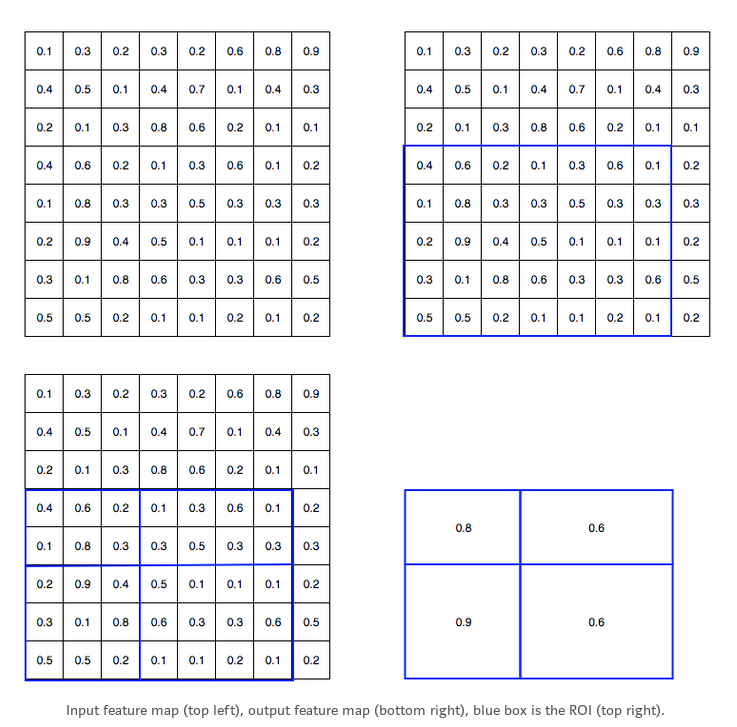
\includegraphics[scale=0.3]{./tex/computer-vision/object-recognition/roi.png}
    \caption{Exemple - RoI Pooling}
    \label{roi}
\end{figure}


\subsubsection{Intersection over Union (IoU)}
Afin d'évaluer la performance des prédictions réaliser dans le cadre des thématiques vues précédemment, il est nécessaire de définir une métrique de performance. En effet, les métriques standards telles que l'Accuracy ou la Précision sont inefficaces pour juger de la validité des \textit{bounding boxes}. Afin de résoudre ce problème, la métrique \textit{Intersection over Union} est utilisée. Une illustration est visible sur la Figure \ref{iouim}.\\

\noindent Supposons une image d'apprentissage. Une \textit{bounding boxes} de référence est définie et l'objectif de notre modèle est de la reproduire. Ainsi, si la \textit{bounding boxes} prédite est strictement identique à la \textit{bounding boxes} d'apprentissage, alors la prédiction peut être jugée comme \textit{parfaite}. Deux \textit{bounding boxes} identiques signifient que leurs coordonnées sont identiques, et de ce fait, il en va de même pour la surface qu'elles englobent. Cette particularité est à l'origine de la métrique IoU.\\

\noindent Considérons l'intersection de deux \textit{bounding boxes}. Une intersection entre la \textit{bounding boxes} prédite et d'apprentissage de même dimension que cette dernière signifie que l'entité a été entièrement détectée. Néanmoins, ce résultat possède une faiblesse majeure car elle ne considère pas la précision de la \textit{bounding boxes} prédite. Ainsi, supposons une image quelconque. Si la \textit{bounding boxes} prédite englobe l'intégralité de l'image, alors l'intersection entre les deux surfaces sera de la dimension de la \textit{bounding boxes} d'apprentissage mais le résultat sera très mauvais. Il faut donc un critère discriminant la précision de la \textit{bounding boxes} prédite. Ce problème est corrigé par la considération de la surface d'union des deux \textit{bounding boxes}. En effet, si les deux \textit{bounding boxes} sont identiques, alors la surface d'union et d'intersection seront identiques. Au contraire, si elles différent, la surface obtenue sera supérieure à la valeur de la \textit{bounding boxes} d'apprentissage. \\

\noindent On obtient donc une relation permettant de considérer ces deux spécificités: $$IoU(s,s')=\frac{s \cap s'}{s \cup s'}$$
Si les deux surfaces sont identiques, alors IoU(s,s')=1 et tend vers 0 lorsqu'elles diffèrent. Il s'agit donc d'une métrique normalisée, ce qui facilite son exploitation. Il est commun de considérer une \textit{bounding boxes} prédite comme de qualité si $IoU(s_{ref},s_{pred}) \geq 0.5$. C'est la valeur de référence pour la plupart des compétitions officielles exploitant cette métrique.

\begin{figure}
    \centering
    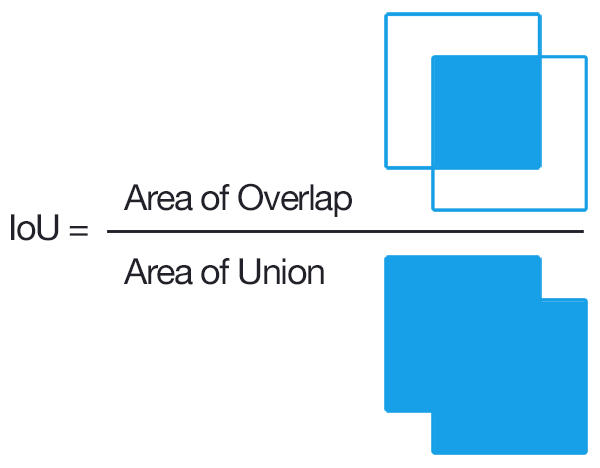
\includegraphics[scale=0.3]{./tex/computer-vision/object-recognition/iou.png}
    \caption{Illustration de la métrique Intersection over Union (IoU)}
    \label{iouim}
\end{figure}

\subsubsection{Non-Max Suppression}
Lors de la prédiction des \textit{bounding boxes}, une même entité peut être associée à plusieurs \textit{bounding boxes}. Ce phénomène est illustrer sur la Figure \ref{nonmaxdetec}. Il est donc nécessaire de filtrer ces différentes prédictions afin de ne garder que les meilleures et associer à une entité, une unique \textit{bounding boxes}. Un algorithme de tri existe et s'appelle \textit{Non-Max Suppression}.\\

\noindent Supposons un problème d'\textit{Object Detection} à 3 classes. Une prédiction de sortie est donc de la forme:
$$y=[p_c, b_x,b_y,b_h,b_l,c_1,c_2,c_3]$$
\noindent Cet algorithme s'effectue en deux étapes. La première est la suppression de toute \textit{bounding boxes} dont la confiance de la détection est inférieure à une valeur-seuil définie (supposons 0.7) donc si $p_c < 0.7$. La seconde étape est une procédure itérative qui réalise la sélection de la meilleure \textit{bounding boxes} pour chaque entité-cible.\\

\noindent Supposons tout d'abord un problème mono-classe (il n'y a donc pas de variable $c_i$ dans le vecteur de prédiction). L'objectif est de supprimer les \textit{bounding boxes}-doublons qui localisent une même entité. Il est donc probable qu'il y est des chevauchements de surface entre chacune de ces \textit{bounding boxes}. L'idée est donc de supprimer les \textit{bounding boxes} qui partagent une trop grande surface soit définir une valeur-seuil pour la valeur de l'IoU. Ainsi, cette partie se découpe en deux phases. Tout d'abord, on choisit la \textit{bounding boxes} avec la confiance la plus importante puis on supprime toutes \textit{bounding boxes} dont l'IoU avec la \textit{bounding boxes} ciblée est supérieure à la valeur-seuil choisie (disons 0.5). Cette étape est ainsi répétée itérativement jusqu'à ce que toute les \textit{bounding boxes} soit traitées (suppression ou préservation).\\

\noindent Dans le cas d'un problème multi-classe, le cycle est séparé selon la classe prédite par la \textit{bounding boxes}. Ainsi, si un IoU entre deux \textit{bounding boxes} est supérieur à la valeur-seuil (0.5) mais que la classe prédite diffère, alors il n'y aura pas de suppression de \textit{bounding boxes}. On réalise donc le cycle en ne considérant que la classe 1, puis on recommence avec la classe 2 etc... Cette spécificité permet de mieux traiter le cas d'entités de nature différente mais proche spatialement\footnote{Par exemple, un cycliste où l'on localise le vélo et l'individu.}. Un exemple concret est visible sur la Figure \ref{nonmaxdetec2}\\

\noindent Néanmoins, une faiblesse majeure existe. En effet, une hypothèse est faite que deux \textit{bounding boxes} qui se chevauchent et de même classe identifient la même entité. Bien que vrai dans de nombreux cas, il y a d'autres cas où c'est problématique, notamment les nuées denses telles qu'une foule d'individus, une nuée d'oiseaux ou d'abeilles par exemple.


\begin{figure}
    \centering
    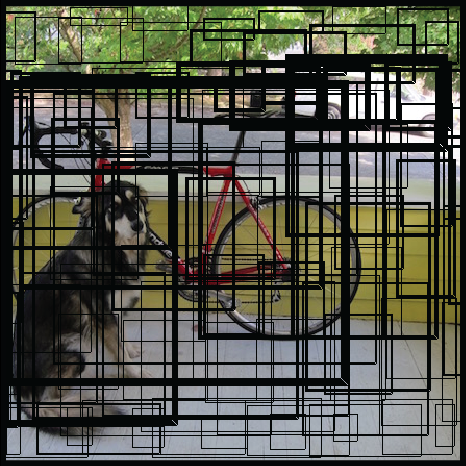
\includegraphics[scale=0.3]{./tex/computer-vision/object-recognition/nonmax.png}
    \caption{Illustration de la problématique de la superposition de bounding boxes}
    \label{nonmaxdetec}
\end{figure}

\begin{figure}
    \centering
    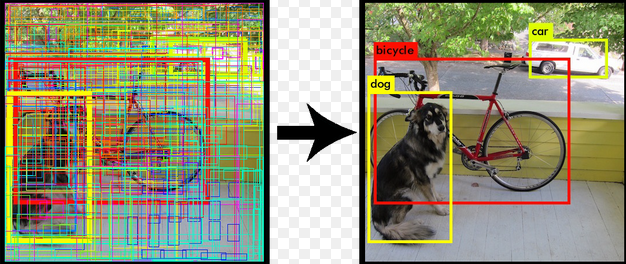
\includegraphics[scale=0.4]{./tex/computer-vision/object-recognition/nonmax2.png}
    \caption{Illustration de Non-Max Detection}
    \label{nonmaxdetec2}
\end{figure}

\subsubsection{Feature Pyramid}
\label{fepyramide}
\textit{Feature Pyramid}\cite{featurepyramide} (FPN) propose une nouvelle méthode d'extraction d'attribut d'une image. En effet, un dilemme existe entre résolution de la \textit{feature map} et l'information sémantique produite. Plus les couches de convolution se succèdent, plus l'information sémantique se développe au détriment de la résolution qui diminue\footnote{Pas de Padding et application de Downsampling récurrente}. Ceci est problématique car ça favorise les entités de grande taille sur l'image au détriment des plus petites qui seraient "noyées" par la perte de résolution. Il est donc nécessaire d'apporter une solution afin de conserver l'information portée par les \textit{feature map} de grande résolution. \\

\noindent \textit{Feature Pyramid Networks} propose une approche pyramidale. Elle se décompose en deux étapes: l'étape \textit{Bottom-up} et l'étape \textit{Top-down}.
\begin{itemize}
    \item \textbf{Bottom-up}: Cette étape est comparable à une succession de couches convolutives standards dont le \textit{stride} augmente de manière à diviser par deux la dimension des \textit{feature map} en sortie. La valeur sémantique des\textit{feature map} augmente au fil des étages de la pyramide mais sa résolution diminue du fait de l'impact des \textit{stride}. Chaque étage peut produire ou une ouplusieurs \textit{feature map}.

    \item \textbf{Top-down}: Cette étape réalise un \textit{Upsampling} sur les \textit{feature map}. La résolution de l'image est grossière\footnote{Le Upsampling ne peut garantir une mise à l'échelle précise} mais l'information sémantique est, quant à elle, forte. Le premier étage de la pyramide (première couche de convolution) n'est pas considéré durant cette étape car trop gourmande en mémoire (et temps de traitement). Chaque étage issu de \textit{Bottom-up} ou \textit{Top-down} traitent des données de même dimension deux à deux.

    \item \textbf{Connexions latérales}: L'étape \textit{Top-down} souffre du \textit{Upsampling} qui ne peut retranscrire la résolution de l'image avec fidélité. Pour corriger ce défaut, des connexions latérales sont produites. Une connexion relie deux étages respectivement, i.e l'étage 3 de \textit{Bottom-up} est lié à l'étage 3 de \textit{Top-down}. Une liaison extrait les \textit{feature map} de l'étage correspondant, réalise une convolution 1*1 afin de contrôler la profondeur et additionne la sortie obtenue avec les \textit{feature map} correspondant sur le cycle \textit{Top-down}.

    \item \textbf{Sortie prédictive}: Les \textit{feature map} issues de l'étape \textit{Top-down} sont soumises à une autre couches de convolution (filtre 3*3) avant d'être exploité par les couches de détection et classification.
\end{itemize}

\noindent Une illustration de cette architecture est visible sur la Figure \ref{fepyr}. \textit{Feature Pyramid} n'est pas un réseau de détection d'entité mais un extracteur d'attributs exploitable par d'autres architectures, notamment par le modèle RetinaNet.

\begin{figure}
    \begin{tabular}{cc}
        a) 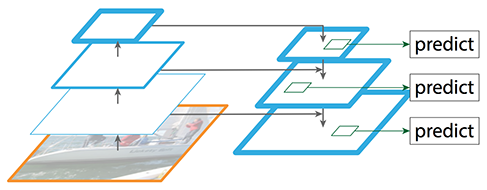
\includegraphics[scale=0.4]{./tex/computer-vision/object-recognition/pyramidfeature.png}& b) 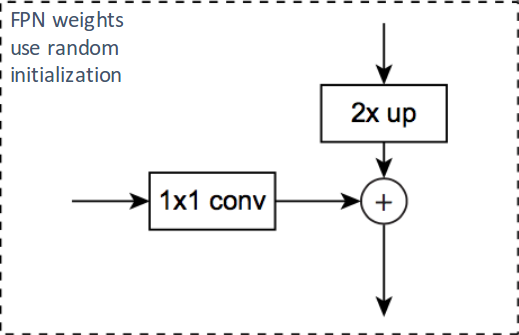
\includegraphics[scale=0.3]{./tex/computer-vision/object-recognition/conneclate.png}
    \end{tabular}
    \caption{Illustration de l'architecture Feature Pyramid: a) Architecture générale b) Architecture des connexions latérales }
    \label{fepyr}
\end{figure}

\paragraph{Amélioration de l'architecture du réseau central}
\paragraph{A faire}
\cite{denet} https://arxiv.org/pdf/1804.06215.pdf

\subsection{Object recognition: méthodes State-of-the-art}
\textbf{Attention}: Cet aperçu de l'état de l'art n'est qu'indicatif et propose quelques approches présentant une efficacité reconnue ou une originalité novatrice (et intéressante à étudier). Il est certain qu'il doit exister d'autres méthodes aux performances au moins similaires.\\

\noindent Il existe deux grandes familles d'algorithmes d'\textit{Object Detection}: \textit{Region based object detectors} et \textit{single shot object detectors}. Ces deux familles ont des algorithmes performants à l'état de l'art bien que leurs approches différent légèrement.\\

\noindent En effet, \textit{Region based object} est caractérisé par le fait qu'un même calcul sur une image puisse être réalisé plusieurs fois au sein d'une prédiction. Par exemple, une même \textit{feature map} peut être exploitée (en partie) plusieurs fois au sein du réseau (lors de la création de la \textit{bounding boxe} et de la classification de l'entité isolée par exemple). Cette tolérance à la redondance de calculs permet de favoriser une précision élevée du réseau mais porte préjudice à sa vélocité. De plus, cette famille d'algorithme est caractérisée par une approche en \textit{bloc}. C'est-à-dire qu'elle accepte l'exploitation d'algorithmes extérieurs et ou de structures parallèles au sein d'un même réseau (par exemple, deux réseaux de neurones). La méthode finale est donc une combinaison de méthodes distinctes. Cette tolérance rend plus difficile l'apprentissage du réseau du fait de la nature différente de ses composants.\\

\noindent \textit{Single shot object}, au contraire, cherche la simplicité et l'unicité. Elle n'exploite une donnée qu'une fois uniquement, ce qui permet une vitesse bien plus importante grâce à la non-redondance de calculs. L'objectif est donc d'unir le réseau de classification et de \textit{Region Proposal} au sein du même réseau. Néanmoins, cette approche tend à rendre le modèle moins robuste bien que les modèles récents s'approchent grandement des performances des \textit{Region based object}. Cette approche tend à donner des réseaux plus \textit{simples} et modulables et semble gagner la bataille en terme de popularité grâce à cette simplicité qui laisse penser qu'elle possède une plus grande marge de progression.\\

\noindent Les méthodes \textit{Region based object} sont principalement \textit{R-CNN}, \textit{Fast R-CNN}, \textit{Faster R-CNN} et \textit{R-FCN}. Les approches \textit{Single shot object} sont \textit{YOLO} et \textit{SSD}.

\subsubsection{R-CNN - Algorithme précurseur}
R-CNN\cite{rcnn} est un algorithme d'\textit{Object recognition} développé en 2014. Son fonctionnement repose sur des méthodes décrites dans la section précédente.\\

\noindent Le réseau se partage en 3 parties indépendantes:
\begin{itemize}
    \item Création de \textit{bounding boxes}: Cette étape est réalisée par une méthode de \textit{Regional Proposal}. \textit{Selective Search} a été choisi par les créateurs de R-CNN. Il y a une création d'environ 2000 \textit{bounding boxes}.

    \item Extraction d'attributs: Les sous-images discriminées par les \textit{bounding boxes}\footnote{Elles représentent une partie de l'image brute initiale} sont analysées par un réseau convolutif déjà pré-entrainé. L'entrée de ce type de réseau est de taille fixe. Il est donc nécessaire de s'assurer que chaque image possède la même dimension. Pour redimensionner les images, une approche par \textit{Warping} ou \textit{Cropping} est utilisée.

    \item Prédiction et affinement: Cette étape réalise 2 actions: Prédire la classe de l'entité présente dans la \textit{bounding boxes} observée\footnote{Dans la majorité des cas, aucune classe n'est représentée car il n'y a pas d'entité présente!} et un affinement de la dimension de la \textit{bounding boxes}.\\

    La classification est réalisée par un modèle indépendant. Dans l'architecture originale, un SVM (\textit{Support Vector Machine\footnote{C'est un algorithme de Machine Learning utilisé pour des problèmes de Classification}}) est utilisé. Le raffinement de la \textit{bounding boxes} est réalisée par un réseau Full-Connected qui est chargé de prédire une nouvelle dimension pour la \textit{bounding boxes}. Ce réseau réalise donc une "correction d'erreur' de la dimension par défaut obtenue par l'algorithme de \textit{Region Proposal}. Un exemple illustratif de ce réseau est visible sur la Figure \ref{rcnn2}.

\end{itemize}

\noindent Un graphique récapitulatif de ce réseau est visible sur la Figure \ref{rcnn1}. Ce réseau possède des résultats remarquables en comparaison des autres méthodes du moment. Néanmoins, du fait des composants indépendants de son architecture, son apprentissage n'est pas aisé et ses prédictions longues à réaliser. Par conséquent, il ne peut pas être exploité dans le cadre du temps-réel.

\begin{figure}
    \centering
    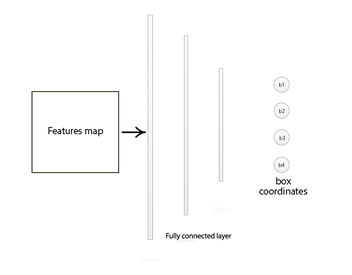
\includegraphics[scale=0.4]{./tex/computer-vision/sota/rcnn2.png}
    \caption{Illustration d'un réseau de prédiction de bounding boxes selon R-CNN}
    \label{rcnn2}
\end{figure}

\begin{figure}
    \centering
    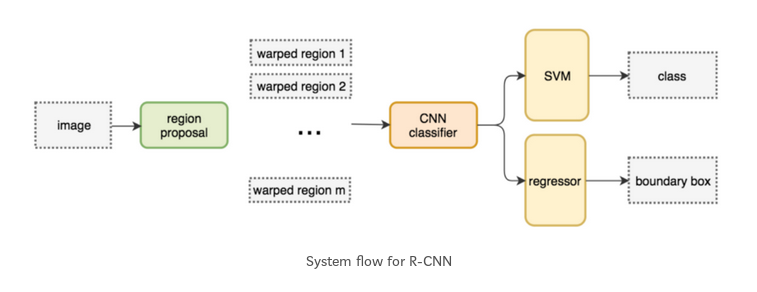
\includegraphics[scale=0.4]{./tex/computer-vision/sota/rcnn1.png}
    \caption{Illustration d'un réseau R-CNN}
    \label{rcnn1}
\end{figure}

\subsubsection{Spatial Pyramid Pooling - Algorithme précurseur}
R-CNN souffre de sa lenteur de prédiction. Cette lenteur est essentiellement due au réseau convolutif appliqué sur chaque \textit{bounding boxes}. En effet, étant donné le recouvrement de nombreuses \textit{bounding boxes}, il y a une redondance de calcul réalisé lors des créations de \textit{feature map}\footnote{Le filtre de convolution va analyser les mêmes pixels plusieurs fois d'où la redondance}. La proposition de \textit{Spatial Pyramid Pooling Network}\cite{sppnet}(SPPnet) est de réaliser l'extraction des \textit{feature map} \textbf{avant} l'application de l'algorithme de \textit{Region Proposal}. Ainsi, l'algorithme de \textit{Region Proposal} va s'appliquer sur la \textit{feature map} de l'image et non l'image originale, permettant ainsi de réaliser l'extraction d'attributs une fois uniquement.\\

\noindent La problématique d'uniformisation des dimensions reste présente. Afin d'uniformiser les \textit{feature map} issues de l'algorithme de \textit{Region Proposal}, SPPnet introduit \textit{Spatial Pyramid Pooling}. Cette méthode exploite une architecture pyramidale basée sur une action de Pooling où chaque étage de la pyramide réalise un Pooling de dimensions différentes sur la \textit{feature map} initiale. Cette méthode permet ainsi d'avoir une sortie de dimension $N*K_i$ avec N, nombre d'étages de la pyramide et $K_i$, nombre de valeurs obtenues par le Pooling. Cette valeur varie pour chaque étage, la dimension de sortie n'est donc pas uniforme selon l'axe de N. Un exemple est visible sur la Figure \ref{spplayer}.\\

\noindent L'architecture de prédiction du réseau est similaire à l'architecure R-CNN. L'apport principal de ce réseau est le gain de temps important par rapport à R-CNN pour une qualité de prédiction similaire. Le réseau convolutif doit être appris en amont. L'architecture de SPPnet ne permet pas son apprentissage. La Figure \ref{sppnet} résume l'architure de SPPnet.

\begin{figure}
    \centering
    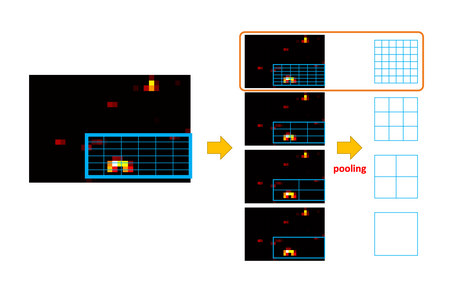
\includegraphics[scale=0.4]{./tex/computer-vision/sota/spplayer.png}
    \caption{Illustration du Spatial Pyramid Pooling}
    \label{spplayer}
\end{figure}

\begin{figure}
    \centering
    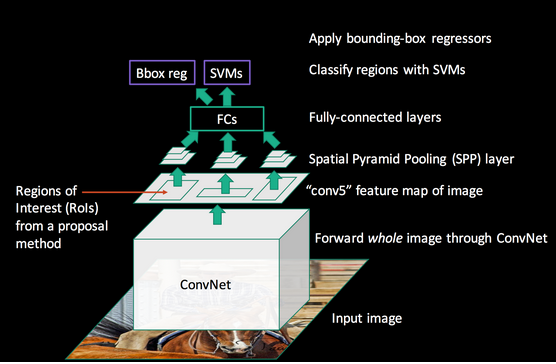
\includegraphics[scale=0.4]{./tex/computer-vision/sota/sppnet.png}
    \caption{Illustration du Spatial Pyramid Pooling Network}
    \label{sppnet}
\end{figure}

\subsubsection{Fast R-CNN - Algorithme précurseur}
Fast R-CNN\cite{fastcnn}, comme son nom l'indique, est une optimisation de R-CNN pour minimiser son temps d'exécution et faciliter son apprentissage. Ces deux améliorations reposent sur 2 spécificités.\\

\noindent Comme SPPnet, Fast R-CNN réalise l'extraction d'attributs par réseau convolutif avant l'exploitation d'un algorithme de \textit{Region Proposal}. L'uniformisation des dimensions est réalisée par \textit{RoI Pooling} (voir Section précédente). Cette uniformisation est comparable à un cas particulier de \textit{Spatial Pyramid Pooling} où la pyramide possède qu'un étage uniquement (voir Figure \ref{fast1}).\\

\noindent La plus-value véritable comparée à SPPnet est le remplacement du SVM par un réseau Full-Connected qui réalisera la classification. Cette modification permet ainsi de réaliser une mise à jour intégrale du réseau (CNN+FC) par rétro-propagation du fait de l'architecture intégralement neuronale. Sans cette modification, le réseau convolutif doit être appris en amont indépendamment du réseau. Seules les couches FC pourraient être entraînées par le biais de la prédiction du correctif des \textit{bounding boxes}. Ce système peut donc exploiter une méthode d'apprentissage unitaire et faciliter son exploitation en unifiant les entités du réseau. L'architecture du réseau et sa structure d'apprentissage sont visibles sur la Figure \ref{fast2}.

\begin{figure}
    \centering
    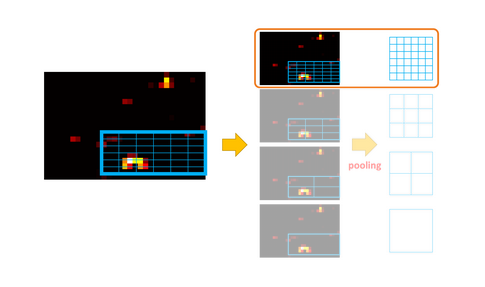
\includegraphics[scale=0.4]{./tex/computer-vision/sota/fast1.png}
    \caption{Analogie de RoI Pooling avec Spatial Pyramid Pooling}
    \label{fast1}
\end{figure}

\begin{figure}
    \centering
    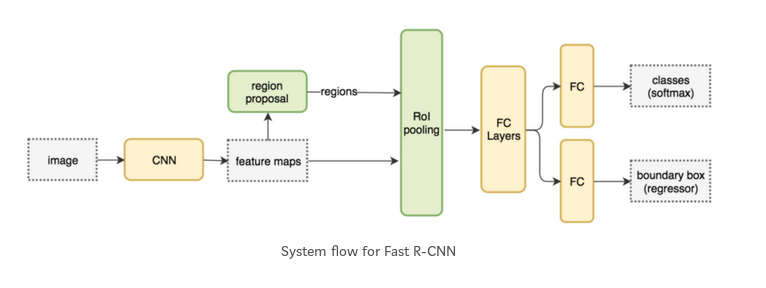
\includegraphics[scale=0.4]{./tex/computer-vision/sota/fastrcnn.png}
    \caption{Illustration du Fast R-CNN}
    \label{fast2}
\end{figure}

\subsubsection{Faster R-CNN}
\label{fastrcnnsec}
Faster R-CNN\cite{fastercnn_deep} est une amélioration de Fast R-CNN. L'idée derrière cette architecture est de s'émanciper de l'algorithme de \textit{Region Proposal} qui était indépendant du réseau jusque-là (utilisation de l'algorithme \textit{Slinding Search}). Cette dépendance est très problématique car il est le facteur limitant à la vélocité du système. Faster R-CNN propose donc une approche qui intègre dans son réseau-même, une méthode de \textit{Regional Proposal} nommée \textit{Region proposal network}(RPN). Cette architecture repose sur l'approche par \textit{Anchor Boxes} (voir Section précédente) et est intégralement convolutif. La sortie de RPN correspond à la confiance en la présence d'une entité ou non sur l'\textit{anchor} et des coordonnées corrigées de l'\textit{anchors} utilisée. Si il y a 9 \textit{anchors}, il y aura K*9*(N+M) valeurs de sortie où K, nombre de case du quadrillage, N nombre de variable pour représenter la confiance\footnote{En général, il n'y a qu'une valeur en sortie} et M, caractéristiques de la fenêtre\footnote{En général, il y a 4 valeurs en sortie}.\\

\noindent La partie prédictive du réseau est similaire à Fast R-CNN (RoI Pooling + classification par réseau Full-Connected). Une autre plus-value du système est de créer une méthode de \textit{Region Proposal} propre à un jeu de données. Du fait que RPN apprend sur le jeu de données d'apprentissage de tout le réseau et non indépendamment, il sera parfaitement adapté et spécialisé à la nature des données observées. Il est intéressant de noter qu'il y a un double ajustement de la dimension des \textit{ bounding boxes}: lors de l'ajustement de l'\textit{anchor} par le RPN et lors de la classification après l'uniformisation des dimensions par RoI.\\

\noindent Une illustration de ce réseau est visible sur la Figure \ref{faster}. Il est un modèle avec l'une des meilleures précisions de l'état de l'art. Il reste néanmoins très lourd et lent, ce qui l'empêche d'être exploitable en temps-réel. Néanmoins, Faster R-CNN a été une amélioration remarquable de l'approche proposée par R-CNN. Un comparatif de performance est visible sur la Figure \ref{compfaster}. D'autres approches sont préférées aujourd'hui car bien plus rapide et avec une qualité de résultat satisfaisante (telles que YOLO ou SSD par exemple). De plus, une faiblesse de ce type d'approche est la séparation des tâches. La séparation entre le réseau qui produit les \textit{bounding boxes} et le réseau prédictif favorise un coût de calculs important lié à la redondance de calculs entre la phase de création des fenêtres et de la classification (les deux réseaux observent la même feature map) d'où les limites de vitesse de ce type de réseau.

\begin{figure}
    \centering
    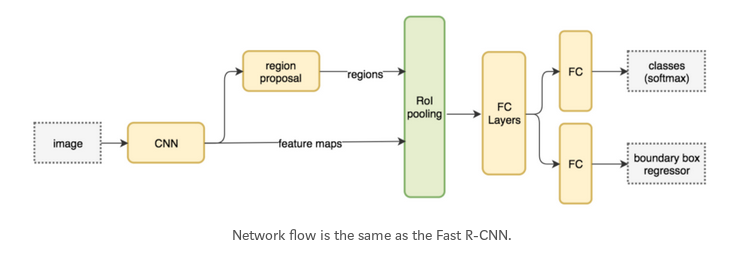
\includegraphics[scale=0.4]{./tex/computer-vision/sota/rpn.png}
    \caption{Illustration du Faster R-CNN}
    \label{faster}
\end{figure}

\begin{figure}
    \centering
    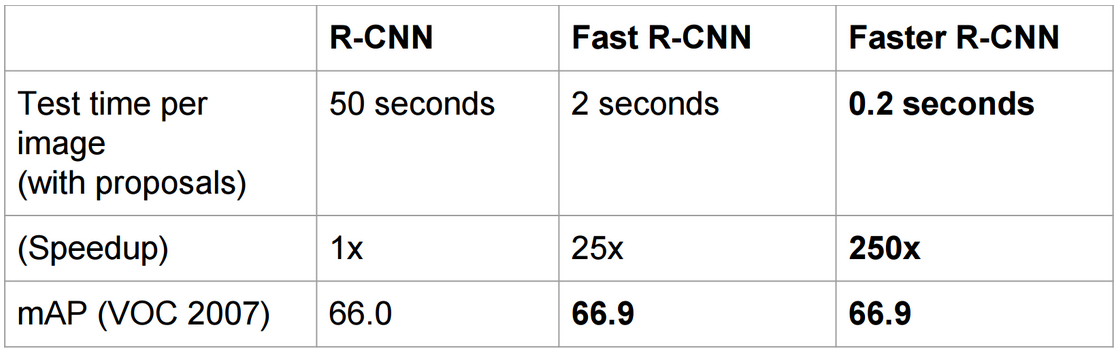
\includegraphics[scale=0.3]{./tex/computer-vision/sota/fas12.png}
    \caption{Comparatif de performance entre R-CNN, Fast R-CNN et Faster R-CNN}
    \label{compfaster}
\end{figure}

%\subsubsection{R-FCN}
%\cite{rfcn}

\subsubsection{Différence principale entre Single shot et Region based}
Faster R-CNN, du fait de son architecture entièrement basée sur des réseaux de neurones, se rapprochent de l'architecture \textit{Single shot}. Néanmoins, une différence majeure est encore présente et repose sur son approche de l'algorithme \textit{Anchors Box}.\\

\noindent Supposons la création de 9 \textit{anchors}, La sortie du RPN associée à Faster R-CNN sera de la forme K*9*(N+M)\footnote{Voir section \ref{fastrcnnsec} pour plus de détails}. N (souvent égal à 1) et M (souvent égal à 4) sont associés à la confiance en la présence d'une entité et à la dimension de la \textit{bounding boxe}. La classification de l'entité est donc complètement ignorée, la sortie se limitant à dire sa confiance en la présence d'une entité sans discrimination. Cette sortie est donc envoyée à un autre "sous-réseau" pour la classification.\\

\noindent Au contraire, dans le cas d'un algorithme \textit{Single shot}, la sortie serait de la forme K*9*(N+M+C) où C, probabilités de classification pour une classe donnée. Cette sortie est donc associée à la fin de la prédiction et donc du réseau prédictif. Il n'y a pas de transfert à un autre sous-réseau de classification. Supposons une \textit{feature map} de dimension 10*10 où 20 classes sont à discriminer avec l'aide de 9 \textit{anchors}. On obtiendra donc pour Faster R-CNN, une sortie de dimension 10*10*9*(1+4) et pour un algorithme \textit{Single shot}, 10*10*9*(1+4+20). Une illustration est visible sur la Figure \ref{singleshot}.\\

\begin{figure}
    \centering
    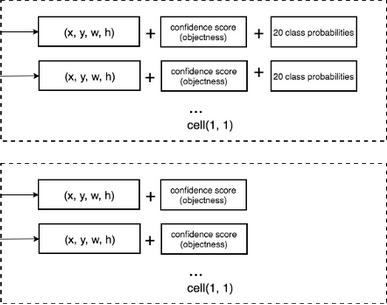
\includegraphics[scale=0.6]{./tex/computer-vision/sota/singleshot.png}
    \caption{Différence de la sortie des couches convolutives entre les approches Single shot et Region based}
    \label{singleshot}
\end{figure}

\noindent Cette différence sur l'aspect prédictif implique une différence majeure: les modèles \textit{Single shot} ont une valeur finie (et identique) de \textit{bounding boxes} définies pour chaque image (en accord avec le quadrillage de l'image\footnote{Cette particularité est expliquée dans les sections qui vont suivre}) alors que les approches \textit{Region based}, de part la séparation des sous-réseaux, permettent la création d'un nombre indéfini de \textit{bounding boxes}. Cette spécificité des modèles \textit{Region based} permet généralement d'obtenir un meilleur taux de détection car le \textit{Rappel} est plus important. Néanmoins, ces modèles sont plus lourds, plus lents et plus sensibles aux problèmes de distributions fortement désiquilibrées entres les classes (notamment entre les classes associées à une entité et la classe générale qui traduit l'absence d'une entité).

\subsubsection{You Only Look Once (YOLO)}
Les méthodes précédentes séparent le réseau de \textit{Region Proposal} du classifier. Une autre approche proposée par YOLO repose  sur l'idée de pouvoir obtenir les \textit{boundary boxes} et les classes directement à partir des \textit{feature map} en un réseau unique. YOLO a été très populaire lors de sa sortie grâce à sa structure \textit{simple} et souple d'utilisation. Aujourd'hui, deux versions ont été réalisées afin d'améliorer les performances de la version initiale. De plus, des versions dites \textit{tiny} du réseau ont été crées pour diminuer l'impact mémoire du réseau et ses exigences matérielles pour réaliser les prédictions. Il s'agit donc de versions idéales pour des systèmes portables et embarqués.

\paragraph{YOLOv1}
La première version de YOLO\cite{yolo_deep} repose sur un réseau convolutif finalisé par deux couches Full-Connected. Le réseau va reproduire le comportement suivant:
\begin{itemize}
    \item L'image d'entrée est divisé selon un quadrillage de dimension S*S. Si le \textit{centre} d'une entité de l'image (défini par le centre d'une \textit{bounding boxes}) est présent dans une des cases du quadrillage, alors cette case est responsable de déterminer la classe de l'objet.

    \item Chaque case prédit K \textit{bounding boxes}, i.e ses coordonnées spatiales (centre(x,y), hauteur et largeur) et son degrés de confiance en la présence d'un objet au sein de cette \textit{bounding boxes}. Le degrés de confiance n'exprime que la probabilité qu'une entité quelconque soit présente. Il n'y a pas de discrimination de la nature de l'entité à ce niveau. Cette valeur, dans le cas idéal, devrait être exprimé selon:\\

    Si aucun objet est présent:
    $$conf(B_i)=0$$
    Si un objet est présent (même partiellement):
    $$conf(B_i)=Pr(entite)*IoU_{Pred,True}$$
    Avec $Pr(entite)$, probabilité qu'une entité soit présente et $IoU_{Pred,True}$, IoU entre la \textit{bounding box} crée par le réseau et la vraie à obtenir. Ainsi, cette valeur permet d'évaluer la présence ou non d'un objet et la surface de l'objet isolé. En effet, une entité peut être détectée mais que partiellement ou au contraire, la surface peut être trop grande.

    \item Chaque case calcule C probabilités de classe $Pr(Classe_i|entite)$. Ainsi, toute \textit{bounding boxes} dont le centre est délimité par cette case sera considérée comme représentative de la classe dont la probabilité est la plus élevée et ce, \textbf{indépendamment} du nombre de \textit{bounding boxes}. Supposons 5 \textit{bounding boxes} dont le centre est dans la case $C_i$ représentant la classe i alors ces 5 \textit{bounding boxes} seront classées comme de la classe i.

    \item La sortie du réseau est donc de la forme: $S*S*(B*5+C)$ avec S*S, nombre de cases du quadrillage, B, nombre de \textit{bounding boxes} et C, nombre de classes discriminées. Dans la version originale, le quadrillage est de 7*7 et chaque case est associée à 2 \textit{bounding boxes} (B=2). 20 classes sont discriminées. La sortie du réseau sera donc de la forme 7*7*(2*5+20).

    \item Les \textit{bounding boxes} sont conservées si la valeur de confiance est supérieure à un seuil. Les \textit{bounding boxes} maintenues sont ensuite filtrées par \textit{Non-Max Suppression}. Une illustration récapitulative est visible sur la Figure \ref{yolov1}.
\end{itemize}

\noindent \textbf{Important}: Les valeurs prédites du centre de la \textit{bounding boxes} sont normalisées. Cette normalisation est \textbf{importante} et nécessaire au bon fonctionnement de YOLO. Le centre de la \textit{bounding boxes} n'est pas prédite de manière \textit{absolue} mais relative à la case à qui elle est associée. Ainsi, les valeurs (x,y) sont comprises entre 0 et 1 relatif à un point de référence défini sur le sommet supérieur gauche par convention. Par exemple, supposons la case (5,5) et supposons un centre idéalement positionné à (5.4, 5.1). La prédiction du réseau ne sera pas (5.4, 5.1) mais (0.4, 0.1). Cette spécificité est capitale pour conserver l'intégrité de l'approche YOLO. En effet, si on réalise une prédiction absolue, il est possible que le centre "quitte" la case associée (par exemple (5.5,6.1). Il y a donc un conflit entre la nouvelle position du centre et la case responsable de la prédiction. Afin de réaliser cette normalisation, les prédictions suivent la relation suivante:
$$ x = \sigma(b_x) + c_x $$
$$ y = \sigma(b_y) + c_y $$
Avec $c_x$, $c_y$ position du sommet supérieur gauche de la case considérée, $\sigma$, fonction sigmoïde\footnote{Elle donne une valeur entre 0 et 1}, (x,y) position réelle du centre et $(b_x,b_y)$, position relative du centre (valeurs prédites).\\

\noindent Le réseau de YOLO est un réseau convolutif inspiré d'une architecture de réseau \textit{Inception} finalisée par deux couches Full-Connected (24+2 couches dans la version originale). Un récapitulatif du réseau est présent sur la Figure \ref{yolov1re} mais pour une présentation détaillée du réseau, veuillez vous référer à l'article de recherche\cite{yolo_deep}. Nous n'approfondirons pas le réseau convolutif qui ne présente pas de particularité notable mais il est intéressant d'étudier les couches Full-Connected du réseau. Comme on peut le voir, la première couche possède 4096 neurones. Or, la sortie finale doit être de dimension 7*7*30, i.e 1470 valeurs\footnote{En effet, la notion de quadrillage est représentée par la dimension de la sortie}.  Il est donc nécessaire de redimensionner la couche. Pour cela, la seconde couche de Full-Connected doit être de dimension 1470 et un redimensionnement de la sortie de cette couche devra être fait afin d'obtenir l'architecture 7*7*30. Une illustration des couches Full-Connected est visible sur la Figure \ref{yolov12}\\

\noindent Une des particularités de YOLOv1 est sa fonction de perte. Elle se présente sous la forme d'une combinaison linéaire de \textit{Squared error} basée sur différentes données. Cette fonction considère la sortie du réseau prédictif. De ce fait, l'intégralité des \textit{bounding boxes} seront considérées\footnote{L'étape de sélection des bounding boxes et l'application de Non-Max Suppression ne sont pas considérées}. Plusieurs spécificités sont à considérer:
\begin{itemize}
    \item Afin d'augmenter la précision des \textit{bounding boxes}, il est utile de pondérer l'erreur associée à la prédictions de la \textit{bounding boxes} par rapport à la classification de l'entité associée. On va donc créer un coefficient $\lambda_{coord}$ (supposons $\lambda_{coord}$=5) qui va pondérer l'erreur de dimension par rapport à l'erreur de classification laissée à 1.

    \item Du fait du nombre important de \textit{bounding boxes} qui ne contiennent pas d'objet, il est important de minorer leurs impacts sur la fonction de coût au risque de voir l'importance des prédictions de \textit{bounding boxes} contenant un objet fortement minorée. En effet, Si l'essentiel des \textit{bounding boxes} sans objet sont bien prédites (c'est souvent plus facile de à réaliser car la discrimination est plus faible pour les \textit{bounding boxes} sans objets) alors une erreur sur une \textit{bounding boxes} contenant un objet sera moins préjudiciable sur le résultat de la fonction de coût car "compensée", ce qui est très problématique. Pour cela, un coefficient noté $\lambda_{noobj}$ est crée et minorera l'erreur correspondant aux \textit{bounding boxes} sans objet. Supposons $\lambda_{noobj}$ égal à 0.5.

    \item Etant donné qu'il n'y a pas de filtrage de \textit{bounding boxes} pour le calcul de l'erreur, il est nécessaire d'isoler la \textit{bounding boxes} qui servira de "référence" pour la prédiction. Afin de la déterminer, on gardera, pour chaque objet identifiée sur l'image d'apprentissage, la \textit{bounding box} possédant le meilleur IoU avec la fenêtre de référence définie sur l'image d'apprentissage. Ainsi, pour 3 entités présentes sur une image, seulement 3 \textit{bounding boxes} seront considérées comme responsable de la prédiction et de ce fait, délimiteur d'un objet. Toutes les autres seront considérées comme négatives. Il y a, bien sûr, un risque important de faux positifs et faux négatifs durant les premières itérations d'apprentissage du réseau.

    \item La classification d'un objet est pertinent si une \textit{bounding box} isole un objet. Si une \textit{bounding box} n'est pas "responsable" de l'isolation d'un objet, la classe prédite par cette \textit{bounding box} n'a pas d'influence sur la fonction de perte. Il en va de même pour la dimension de la fenêtre définie. Ainsi, pour une \textit{bounding box} non responsable de la détection d'une image, seule la valeur de confiance en la présence d'un objet est considérée alors que pour une \textit{bounding box} qui est responsable de la détection d'un objet, la dimension de la fenêtre et la classification sont considérées.

    \item \textit{Square Error} est convexe et présente donc une caractéristique intéressante dans le cadre d'une optimisation. Néanmoins, elle favorise la correction des grandes erreurs et non des petites du fait de la puissance. Cet aspect est problématique car elle favorisera la correction des erreurs associées à de grandes \textit{bounding boxes} et tolérera plus facilement les erreurs sur des petites car l'échelle de la taille des erreurs sera "différente". Cet aspect est partiellement corrigé en considérant la racine carré de la valeur à comparer (hauteur et largeur) et non la valeur réelle. Cette imperfection participe à la faiblesse de YOLOv1 à la détection d'entité de petite dimension.
\end{itemize}

\noindent En considérant ces caractéristiques, la fonction de coût est donc de la forme\footnote{La forme peut impressionner mais elel est facilement compréhensible. Seules les notations sont lourdes !}:
\begin{itemize}
    \item \textit{Bounding boxes} \textbf{responsables} de la détection d'un objet:\\
    \begin{itemize}
        \item \textbf{Dimension}: Centre et Hauteur/Largeur:\\

        Pour $\mathds{1}_{ij}^{obj}=1$ si la \textit{bounding box} est \textbf{responsable} de la détection d'un objet (0 sinon):\\

        $\mathcal{L}_1=\lambda_{coord}\sum_{i=0}^{S^2}\sum_{j=0}^{B}\mathds{1}_{ij}^{obj}[(x_i-\hat{x}_i)^2+(y_i-\hat{y}_i)^2]$ \\
        $\mathcal{L}_2=\lambda_{coord}\sum_{i=0}^{S^2}\sum_{j=0}^{B}\mathds{1}_{ij}^{obj}[(\sqrt{w_i}-\sqrt{\hat{w}_i})^2+(\sqrt{h_i}-\sqrt{\hat{h}_i})^2]$\\

        \item \textbf{Classification}: Confiance + probabilités de classe:\\

        $\mathcal{L}_3=\sum_{i=0}^{S^2}\sum_{j=0}^{B}\mathds{1}_{ij}^{obj}(C_i-\hat{C}_i)^2$\\
        $\mathcal{L}_4=\sum_{i=0}^{S^2}\mathds{1}_{ij}^{obj}\sum_{c \in classes}(p_i(c)-\hat{p}_i(c))^2$\\
    \end{itemize}

    \item \textit{Bounding boxes} \textbf{non responsables} de la détection d'un objet:\\
    \begin{itemize}
        \item \textbf{Classification}: Confiance:\\

        Pour $\mathds{1}_{ij}^{noobj}=1$ si la \textit{bounding box} n'est \textbf{responsable} de la détection d'un objet (0 sinon):\\

        $\mathcal{L}_5=\lambda_{noobj}\sum_{i=0}^{S^2}\sum_{j=0}^{B}\mathds{1}_{ij}^{noobj}(C_i-\hat{C}_i)^2$\\
    \end{itemize}

    \item \textbf{Fonction de perte totale}:\\

    $\mathcal{L}_{total}=\mathcal{L}_1+\mathcal{L}_2+\mathcal{L}_3+\mathcal{L}_4+\mathcal{L}_5$\\
\end{itemize}

\noindent Cette approche présente trois défauts significatifs. Une \textit{bounding boxes} dont le centre est dans une case sera associée à la classe prédite par cette case. Cette contrainte spatiale forte est très préjudiciable en cas d'objets de différentes natures proches. En effet, si deux objets distincts sont proches et donc, que le centre des \textit{bounding boxes} associées sont au sein d'une même case, la prédiction de la classe ne sera pas capable de prédire deux classes distinctes, ce qui produira une erreur de prédiction. De même, chaque case définit B \textit{bounding boxes}. De ce fait, seulement B \textit{bounding boxes} peuvent avoir un centre dans une case, ce qui provoque une limite spatiale au nombre d'entités détectables (S*S*B). Ce modèle est donc peu robuste pour détecter les entités (de même nature) proches et en masse telles que les nuées d'oiseaux ou une foule d'individus par exemple. Pour finir, cet algorithme est très sensible aux dimensions de \textit{bounding boxes} \textit{exotiques}\footnote{YOLO possède de grandes difficultés à détecter des entités de petites tailles}. Il est très dépendant des \textit{bounding boxes} du jeu d'apprentissage, ce qui peut être dangereux avec un jeu de données faiblement représentatif. Ses capacités de discrimination, du fait de l'architecture du réseau choisi (beaucoup de \textit{downsampling}), tend à être grossières. Un risque de faible généralisation est donc probable, de même que des approximations de calculs de dimensions des \textit{bounding boxes}. Une dépendance au jeu de données d'apprentissage semble donc très (trop) importante malgré une efficacité très correcte de l'algorithme.

\begin{figure}
\centering
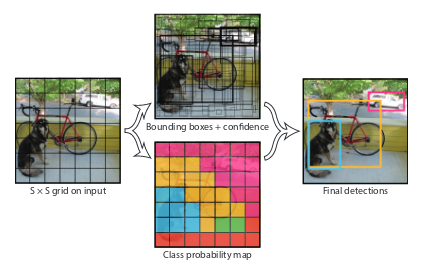
\includegraphics[scale=0.4]{./tex/computer-vision/sota/yolov1.png}
\caption{Fonctionnement général de l'algorithme YOLOv1}
\label{yolov1}
\end{figure}

\begin{figure}
\centering
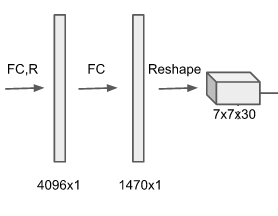
\includegraphics[scale=0.4]{./tex/computer-vision/sota/yolov12.png}
\caption{Architecture des couches Full-Connected de l'algorithme YOLOv1}
\label{yolov12}
\end{figure}

\begin{figure}
\centering
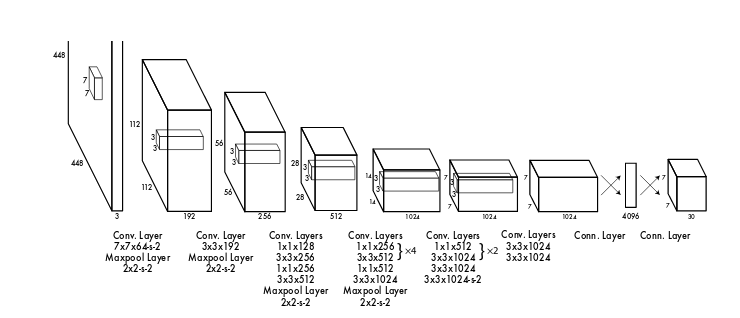
\includegraphics[scale=0.6]{./tex/computer-vision/sota/yolov1rez.png}
\caption{Architecture de l'algorithme YOLOv1}
\label{yolov1re}
\end{figure}

\paragraph{YOLOv2 - YOLO9000}
Afin d'améliorer le modèle initial de YOLO, une version 2 a été crée et appelée (sobrement) YOLO9000\cite{yolov2_deep}. Cette amélioration rend le modèle plus rapide, plus précis et généralise la détection à 9000 classes au lieu de 20.\\

\noindent YOLOv1 réalise un nombre significatif d'erreur de localisation durant ses prédictions. De même, son \textit{Rappel} (Recall) est trop faible comparé aux méthodes de \textit{Region Proposal} classiques\footnote{Notamment utilisées par Faster R-CNN}. Afin d'améliorer le modèle, il a donc été préféré d'améliorer la localisation et la détection d'entité au détriment de la classification.\\

\noindent Afin d'améliorer ces caractéristiques, différents ajouts ont été faits. YOLO9000 utilise \textit{Batch Normalization} après chaque couche de convolution. Afin d'être plus robuste dans la détection, un pré-apprentissage\footnote{Il s'agit de l'entrainement des couches convolutives d'extraction d'informations avant de faire l'apprentissage spécifique de détection} à de multiples résolutions est réalisé (224*224 puis 448*448). Ceci permet d'améliorer le modèle sur la gestion d'images à "haute" résolution. En effet, YOLOv1 réalisait un apprentissage sur des images 224*224 avant de se mettre à l'échelle soit 448*448 mais cette approche ne permettait pas une évolution efficace des extracteurs d'informations des couches convolutives. Un double apprentissage avec YOLO9000 compense cette faiblesse. De plus, la dimension du quadrillage passe de 7*7 à 13*13, ce qui permet une bien meilleure discrimination des entités, notamment groupées. Une approche un peu \textit{tricky} a été faite. En effet, 13 étant impair, le quadrillage possède une case centrale. En générale, une image a tendance à posséder une entité en son centre (ou proche). Il est donc intéressant de pouvoir la détecter sans courir le risque d'un décalage associé à un problème de centre d'\textit{anchor} légèrement décalé. une illustration présente le problème sur la Figure \ref{yolov2odd}.\\

\begin{figure}
\centering
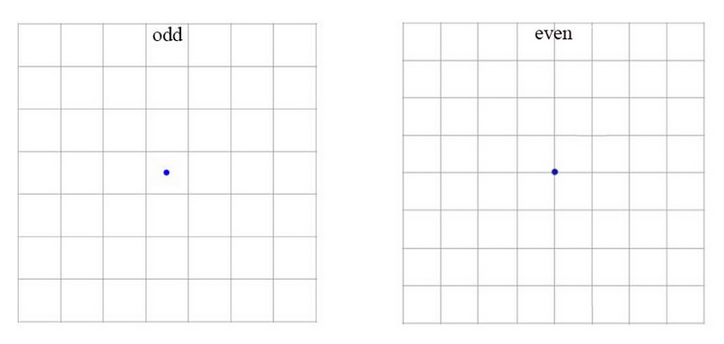
\includegraphics[scale=0.4]{./tex/computer-vision/sota/odd.png}
\caption{Différence de centre entre un quadrillage pair et impair}
\label{yolov2odd}
\end{figure}

\noindent Pour compenser le problème de faible \textit{Rappel}, YOLO9000 va exploiter l'approche par \textit{Anchor boxes} proposée par Faster R-CNN. Cette approche est très bénéfique car elle permet une classification d'entités variées au sein d'une même case du quadrillage. En effet, chaque \textit{anchor} est indépendante et peut prédire une classe distincte. Ainsi, si 9 \textit{anchors} sont présentes sur une même case, alors 9 entités peuvent avoir leur centre localisé sur une même case et être classées selon des classes différentes. Ainsi, il n'y a plus de prédictions "directes" des dimensions de la \textit{bounding box} mais des prédictions d'\textit{offset} d'une dimension pré-établie. Ce travail est plus facile à apprendre pour le réseau de neurones mais diminue la précision du modèle. La diminution est négligeable alors que le \textit{Rappel} augmente significativement. Dans le cadre de YOLOv2, il y a 5 \textit{anchors} par case. \\

\noindent Tout comme pour YOLOv1, le centre est relatif à la case associée. Par contre, la dimension de la \textit{bounding box} sera relative à la dimension de l'\textit{anchor}. On obtient donc:
$$ x = \sigma(b_x) + c_x $$
$$ y = \sigma(b_y) + c_y $$
$$ h = p_he^{th}$$
$$ l = p_le^{tl}$$
$$Pr(entite)*IoU(box,entite)=\sigma(t_0)$$
Avec $c_x$, $c_y$ position du sommet supérieur gauche de la case considérée, $\sigma$, fonction sigmoïde\footnote{Elle donne une valeur entre 0 et 1}, (x,y) position réelle du centre et $(b_x,b_y)$, position relative du centre (valeurs prédites). $p_h$ et $p_l$ correspondent respectivement à la hauteur et à la largeur de l'\textit{anchor}. $t_h$ et $t_l$ sont les prédictions associées aux offset des dimensions de l'\textit{anchor}. $t_0$ est la valeur prédite de la confiance d'une \textit{anchor} en la présence d'une entité. Un exemple est visible sur la Figure \ref{yolov2box}.\\

\begin{figure}
\centering
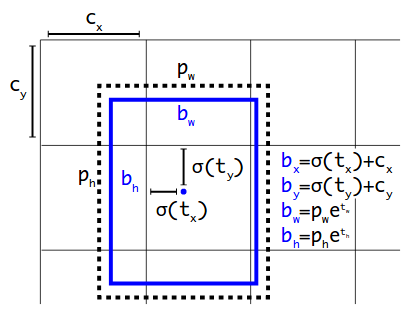
\includegraphics[scale=0.6]{./tex/computer-vision/sota/anchorbox.png}
\caption{Conversion des prédictions du réseau YOLOv2 selon l'anchor associée}
\label{yolov2box}
\end{figure}

\noindent Les \textit{anchors} sont, à la base, prédéfinies manuellement. Il peut être difficile de définir des dimensions capables de discriminer l'essentiel des entités qu'on cherche à détecter. Bien que des dimensions préféfinies aient déjà fait leurs preuves dans divers contextes, YOLOv2 fait le choix de définir des dimensions en adéquation avec le jeu de données d'apprentissage. Pour cela, il va utiliser l'algorithme \textit{K-means}\cite{kmeans}. Pour éviter la problématique de tolérance associée aux faibles dimensions, la métrique euclidienne n'est pas exploitable. Une autre a donc été crée pour corriger ce défaut et repose sur IoU. Elle est définie par:
$$d(box, centroid)=1-IoU(box,centroid)$$

\noindent Afin de considérer la possibilité de présence d'entités de tailles différentes, YOLOv2 va \textit{additionner} des \textit{feature map} à différents niveaux du réseau afin de considérer différentes échelles de dimensions. Ainsi, un comportement similaire à l'addition à la fin d'un block \textit{ResNet} est réalisée. Un exemple illustratif de cette approche est visible sur la Figure \ref{yolov2net}. Il est \textbf{important} de constater que les couches Full-Connected  en fin de réseau ont été remplacées par des couches convolutives, ce qui favorise la vélocité du système.\\

\noindent Par ailleurs, YOLO9000 propose une nouvelle approche afin d'unir différents jeux de données. Dans le cadre de YOLO9000, il s'agit d'imageNet et COCO. Nous ne détaillerons pas cette méthode qui sort du cadre de ce cours. Pour plus d'informations sur cette méthode, référez-vous à l'article associé \cite{yolov2_deep}. YOLOv2 et YOLO9000 sont strictement identiques si ce n'est la différence associée à la méthode d'union des deux jeux de données et de l'apprentissage associé qui s'en voit légèrement modifié.

\begin{figure}
\centering
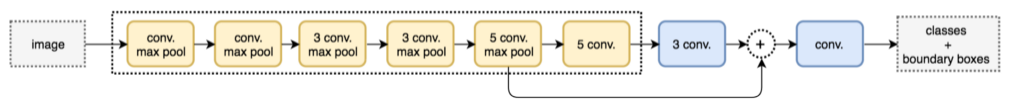
\includegraphics[scale=0.4]{./tex/computer-vision/sota/yolov2net.png}
\caption{Architecture du réseau convolutif YOLOv2}
\label{yolov2net}
\end{figure}

\paragraph{YOLOv3}
La version la plus récente est YOLOv3\cite{yolov3}. Cette amélioration vise à améliorer les performances de prédiction du réseau mais la rapidité de prédiction est diminuée à cause de la complexité grandissante du réseau\footnote{La logique de simplicité et d'autonomie initiale du réseau semble ne plus être un critère décisif des chercheurs}.\\

\noindent Bien que YOLOv2 ait des résultats meilleurs sur cette thématique, la détection des entités de petite taille reste problématique. Cela est due aux \textit{Downsampling} du réseau qui extrait la sémantique de l'image mais nuit à la "résolution" de l'image, ce qui accentue la perte des informations "discrètes" associées à des entités de petites tailles.\\

\noindent Pour corriger ce défaut, plusieurs modifications ont été faites:
\begin{itemize}
    \item \textbf{Architecture interne du réseau approfondie}: Le réseau YOLO était \textit{primaire}. Relativement peu profond, il n'utilisait pas de composantes caractéristiques des réseaux de l'état de l'art. Avec YOLOv3, cette faiblesse n'est plus d'actualité: ajout de \textit{résidus} par addition et concaténation (\textit{skip-layer}), ajout de \textit{Upsampling}, ajout de profondeur (passage de 53 à 106 couches\footnote{D'où la plus grande lenteur du réseau comparé à YOLOv2}). Ces particularités apportent différentes plus-values:
    \begin{itemize}
        \item \textbf{Profondeur du réseau}: L'ajout de couches de convolution permet d'améliorer l'extraction d'attributs des images et, de ce fait, la qualité de la prédiction. Néanmoins, l'impact sur le temps de prédiction est à considérer\footnote{Tout n'est que jeu de compromis...}.

        \item \textbf{Skip-layer et résidus}: Dans les premières couches de convolutions, des \textit{résidus} sont transférés afin de maintenir la bonne cohérence des données dans les différentes couches successives\footnote{Voir ResNet pour plus de détails sur la notion de résidus}. De même, la présence de \textit{Skip-layer} permet de conserver un bon équilibre entre l'information sémantique obtenue par \textit{Downsampling} et l'information détaillée des \textit{feature map} issues des couches précédentes.

        \item \textbf{Upsampling}: Le réseau exploite des \textit{feature map} de différentes dimensions. L'utilisation de \textit{résidus} et de \textit{skip-layer} peut être difficile dans les cas d'opérations sur des \textit{feature map} de dimensions différentes. Afin de les mettre à la même échelle, les \textit{feature map} reçoivent un \textit{Upsampling}. La méthode de \textit{Upsampling} n'est pas explicitée\footnote{A confirmer par une lecture très minutieuse} dans l'article de recherche. Il est donc nécessaire de la choisir selon votre sensibilité personnelle.
    \end{itemize}

    \item \textbf{Prédiction sur 3 échelles}: Alors que YOLOv1/2 réalisait la détection sur un set unique de \textit{feature map}, YOLOv3 le fait sur 3 sets distincts à des échelles différentes (quadrillage appliqué à l'image de différentes dimensions). Plus le \textit{Downsampling} est réalisé au cours du réseau, plus la sémantique de l'image est extrait. Cependant, on perd les détails de l'image et de ce fait sa capacité de détection des petites entités. Afin de corriger cela, une extraction de \textit{feature map} sur 3 sections différentes du réseau permet de réaliser une détection à 3 échelles différentes et ainsi détecter (en simplifiant grossièrement) les entités de petites, moyennes et grandes tailles. Le fonctionnement suit l'idée apportée par les \textit{Feature Pyramid Networks}\footnote{Pour plus d'informations, voir Section \ref{fepyramide}} (FPN).\\

    \item \textbf{Anchor boxes}: 9 \textit{anchors} sont utilisées par YOLOv3. Ces \textit{anchors} sont réparties sur les 3 sorties prédictives. Ainsi, pour chaque sortie, 3 \textit{anchors} sont réparties et appliquées respectivement\footnote{Les 9 anchors ne sont donc pas appliquées sur toutes les feature map}\footnote{On peut considérer qu'il y a 3 anchors fondatrices qui sont mises à l'échelle de différentes manières}. Malgré le fait qu'il n'y ait que 3 \textit{anchors} (5 pour YOLOv2), la présence de 3 sorties prédictives à des échelles bien plus précises (dimension du quadrillage supérieure à 13*13) provoque la création d'un nombre bien plus important de \textit{bounding boxes}. YOLOv3 prédit environ 10x le nombre de \textit{bounding boxes} prédit par YOLOv2.

    \item \textbf{Multi-label}: Il est possible qu'une entité ait plusieurs labels. Par exemple, une femme peut être labellisée \textit{Individu} et \textit{femme}. Avec YOLOv1 et YOLOv2, la classe d'une entité est unique, ce qui est très limitant. Cette limite est due à l'utilisation de la fonction d'activation \textit{Softmax} en sortie prédictive, ce qui produit une prédiction unique (prédiction exclusive). Pour corriger ce défaut, chaque classe est prédite selon une régression logistique\footnote{Comparable à la sigmoïde}, ce qui permet un multi-label pour la classification.

    \item \textbf{Fonction de coût}: La fonction de coût est modifiée pour ses composantes probabilités (confiance et probabilité conditionnelle de classe). L'approche par \textit{Squarred error} n'est pas très performante dans le cadre de comparaison de probabilités. Pour corriger ce défaut, l'utilisation de la \textit{Cross-Entropy} permet d'améliorer les performances de cette fonction.
\end{itemize}

\noindent Une illustration du réseau YOLOv3 est visible sur la Figure \ref{yolov3net}. En considérant la métrique de validation à un IoU de 0.5\footnote{Si l'Iou est supérieur ou égal à 0.5, la prédiction est jugée bonne. C'est une convention pour les compétition d'analyse d'images}, YOLOv3 a des résultats qui dépassent SSD et qui rivalisent avec RetinaNet. Cependant, si le seuil du critère de l'IoU augmente, YOLOv3 perd grandement en performances, ce qui traduit que ce réseau manque de précision dans la prédiction de ses \textit{bounding boxes}. De plus, dans les versions initiales, YOLO avait du mal avec les entités de petites tailles. Avec YOLOv3, les performances pour les entités de petites tailles a augmenté mais la prédictions des entités de tailles intermédiaires et grandes a significativement diminué. Un travail important reste à faire sur la précision de la prédiction. Néanmoins, le réseau reste remarquablement rapide comparé à ses concurrents, ce qui fait de YOLOv3, une alternative parfaitement viable et exploitable\footnote{D'un point de vue métier, les performances sont à la hauteur des attentes. Il est important de savoir que le référentiel n'est pas la performance applicative mais la performance absolue du modèle contre les autres existants, ce qui peut être contre-productif dans le cadre d'une production du modèle au niveau industriel. En effet, un modèle n'a pas à être forcement le "meilleur" au niveau des benchmarks pour être pertinent. De nombreux autres paramètres sont à considérer.} pour les situations nécessitant une vitesse de prédiction élevée comme le \textit{Tracking}.

\begin{figure}
\centering
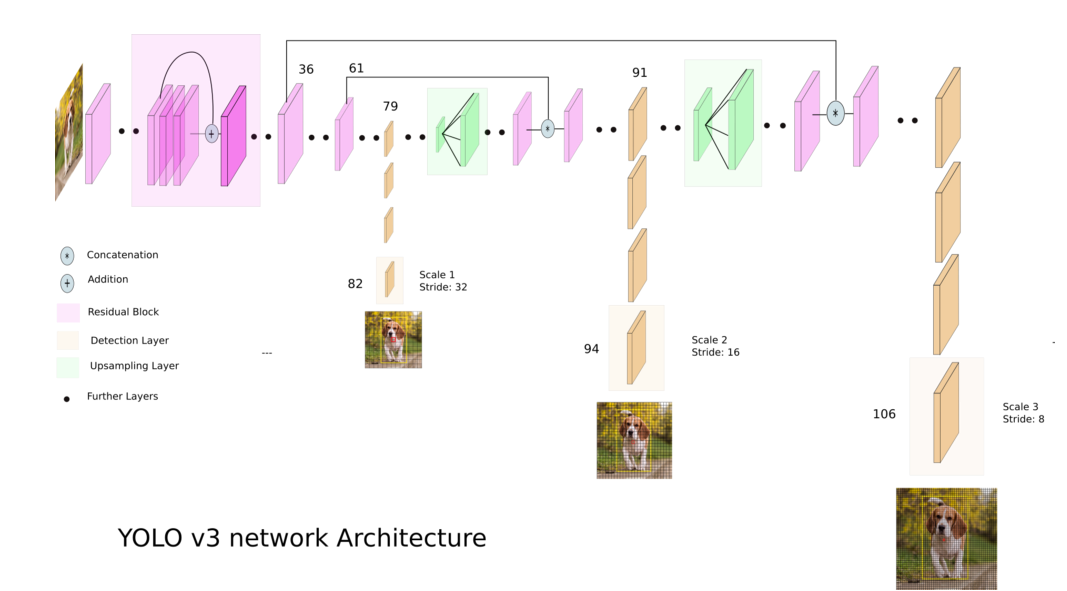
\includegraphics[scale=0.4]{./tex/computer-vision/sota/yolov3.png}
\caption{Architecture du réseau convolutif YOLOv3}
\label{yolov3net}
\end{figure}

\subsubsection{Single Shot MultiBox Detector (SSD)}
SSD est un concurrent de YOLO. Longtemps considéré comme plus performant, les dernières versions de YOLO tendent à relancer la concurrence entre les deux approches tant les performances sont du même ordre de grandeur.
\paragraph{SSD}
Le nom complet du réseau SSD\cite{ssd_deep} traduit les spécificités de son architecture. En effet, SSD est un algorithme \textit{Single Shot}, i.e il réalise la tâche de classification et de localisation sur une même étape \textit{Forward}. La prédiction des \textit{bounding boxes} repose sur l'approche \textit{MultiBox}\cite{multibox} et il réalise une tâche d'\textit{Object Detection} d'où \textit{Detector}.\\

\noindent La version original de SSD repose sur l'architecture VGG-16 où les couches Full-Connected ont été supprimé. En effet, nous n'exploitons que les capacités d'extraction d'attributs de ce réseau et non sa capacité prédictive. SSD se démarque de YOLO par son approche de \textit{détection multi-échelle}. En effet, au lieu de réaliser une prédiction sur un seul set de \textit{feature map}, SSD va extraire des \textit{feature map} à différentes échelles et réaliser une prédiction distincte pour chacun de ces sets. L'architecture du modèle prédictif (convolutif) est différente pour chaque set de \textit{feature map}, ce qui contourne la problématique de dimension des \textit{feature map}. Une illustration du réseau SSD est visible sur la Figure \ref{ssdnet}.\\

\noindent La prédiction des \textit{bounding boxes} suit l'architecture \textit{MultiBox}. Contrairement aux approches standards, \textit{MultiBox} propose une architecture par flux parallèles comparable à l'approche \textit{Inception}. Ainsi, à partir d'un même set de \textit{feature map}, plusieurs prédictions sont réalisées selon des méthodes d'extractions d'attributs variables (couches de convolutions différentes et distinctes). Cette méthode est ainsi plus robuste car elle permet une analyse plus fine des \textit{feature map} et de ce fait, une meilleure prédiction. Un exemple illustratif de \textit{MultiBox} est visible sur la Figure \ref{multiboxnet}.\\

\noindent SSD repose sur l'approche \textit{Anchor box}\footnote{Cette approche est récurrente. Nous ne la détaillerons pas ici. Elle est similaire à celle exploitée par Faster R-CNN}. Ainsi, chaque prédiction est composée de l'offset de la \textit{bounding box} de référence (l'\textit{anchor}) et des probabilités de classes soit (c+4)*k avec c, nombre de classes (contenant la classe \textit{background} qui correspond à aucune classe représentée) et k, nombre d'\textit{anchor}. SSD utilise 6 \textit{anchors} par case.\\

\noindent La fonction de perte de SSD est de la forme:
$$L(x,c,h,l)=\frac{1}{N}(L_{conf}(x,c)+\alpha L_{loc}(x,h,l))$$
Avec $L_{conf}$, fonction d'évaluation de la classification, $L_{loc}$, fonction d'évaluation de la localisation, N nombre de \textit{bounding boxes} conservées et $\alpha$, coefficient de pondération entre la classification et la localisation. C'est un hyperparamètres. $L_{conf}$ repose sur la fonction \textit{Cross-Entropy} pour évaluer la classification et $L_{loc}$ sur \textit{Smooth-L1} pour la localisation. Pour rappel, \textit{Smooth-L1} est définie par:
$$smooth_{L1}(x)=\left\{ \begin{array}{ll} 0.5x^2 \ if \ |x| < 1\\ |x|-0.5 \ otherwise \end{array} \right. $$

\noindent L'utilisation de \textit{Smooth-L1} permet une plus grande souplesse d'apprentissage. En effet, il n'est pas nécessaire d'avoir une précision au pixel-près, ce que favorise la norme L2. Cette contrainte peut être trop forte et limiter l'apprentissage sans réel bénéfice pour l'oeil humain et l'exploitation métier. Pour plus de détails sur la fonction de perte de SSD, référez-vous à l'article de recherche \cite{ssd_deep}. Étant donné le nombre significativement plus grand du nombre de \textit{bounding boxes} négatives, il est nécessaires de limiter leurs utilisations durant l'apprentissage pour conserver un équilibre entre \textit{bounding boxes} positives et négatives. Pour corriger ce défaut, SSD trie les valeurs de la fonction de confiance ($L_{conf}$) pour chaque \textit{anchor} par ordre décroissant et sélectionne ces valeurs de manière à conserver un ration 3:1 entre positifs et négatifs pour l'apprentissage. Cette approche est appelée \textit{Hard Négative Mining}.\\

\noindent Les créateurs de SSD conseille l'utilisation de \textit{Data Augmentation} pour renforcer l'apprentissage et rendre le modèle plus robuste. Leur algorithme de génération de données repose sur l'exploitation de la métrique IoU pour créer différentes sous-images conservant une valeur minimum d'IoU. Cette méthode peut être pratique pour apprendre à détecter des entités partielles, détériorées ou de caractéristiques légèrement différentes de celles présentes dans le jeu de données d'apprentissage.

\begin{figure}
\centering
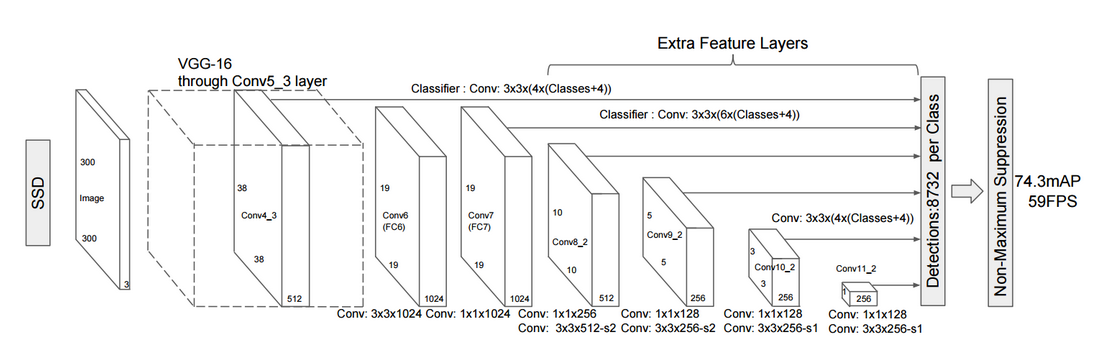
\includegraphics[scale=0.4]{./tex/computer-vision/sota/ssdpic.png}
\caption{Architecture du réseau SSD}
\label{ssdnet}
\end{figure}

\begin{figure}
\centering
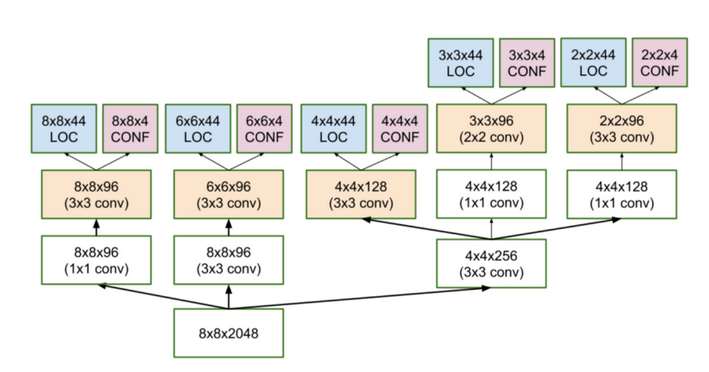
\includegraphics[scale=0.4]{./tex/computer-vision/sota/multibox.png}
\caption{Architecture de Multibox}
\label{multiboxnet}
\end{figure}

\paragraph{Tiny SSD}
Les modèles de Deep Learning sont lourds et exigeants en terme de matériels. Cette contrainte est une problématique récurrente pour implémenter ce type de modèle sur des supports de faibles capacités tels que l'embarqué. Pour répondre à cette contrainte, une version plus légère de SSD a été conçue: Tiny SSD: \cite{tinyssd}.\\

\noindent Ce modèle repose sur l'exploitation de l'architecture \textit{SqueezeNet} et de ses \textit{Fire Module}\footnote{La description détaillée de cette architecture est disponible dans la Section \ref{squeezesect}}. Hormis cette particularité, il n'y a pas de nouveauté significative. Pour plus de détails sur l'architecture du modèle, veuillez consulter l'article associée. L'architecture du réseau est le fruit d'une optimisation soutenue entre exploitation des \textit{Fire Module} et des couches de convolution classiques. Il est donc pertinent de suivre à la lettre, le modèle décrit pour une future implémentation.\\

\noindent Ce modèle est remarquable pour l'embarqué du fait de ses performances et de sa taille. En effet, son concurrent direct (Tiny YOLO) est environ 30x plus lourd (60.5Mo contre 2.3Mo) tout en ayant une performance moins élevée (57.1\%\footnote{Métrique mAP sur VOC 2007} contre 61.3\%).

\paragraph{Deconvolutional Single Shot Detector (DSSD)}
\textit{Deconvolutional Single Shot Detector}\cite{dssd} est une amélioration importante de SSD. Ses deux principales innovations sont le remplacement du modèle VGG par un ResNet (Residual-101) et l'utilisation de \textit{déconvolutions} avec application de \textit{skip-layer}.\\

\noindent Le réseau initial de DSSD est comparable au modèle SSD. Sur la dernière couche de convolution du modèle SSD, le \textit{Downsampling} a permis de produire une image avec une forte explication sémantique mais une faible résolution de l'image. Comme décris précédemment, SSD réalise une extraction de \textit{feature map} sur les dernières couches du réseau afin d'obtenir différentes échelles et ainsi améliorer la prédiction. Bien qu'efficace, cette méthode n'exploite pas les capacités explicatives obtenues par les dernières couches de convolution. En effet, les \textit{feature map} sont extraites \textbf{avant} la (ou les) dernière couche de convolution du réseau. L'idée de DSSD est de ne pas perdre la capacité explicative obtenue lors des dernières couches de convolution. Il ne va donc pas extraire les \textit{feature map} avant ces couches mais \textbf{après}. Pour cela, il est nécessaire d'appliquer une méthode pour redimensionner les \textit{feature map} (\textit{Upsampling}) tout en leur redonnant l'information associée à la résolution de l'image perdue durant l'extraction de la semantique de l'image. Pour cela, DSSD exploite donc la \textit{Déconvolution}\footnote{Ne pas oublier que ce nom est un abus de langage !} pour remettre à l'échelle et des \textit{skip-layer} pour réintroduire l'information de résolution de l'image.\\

\noindent L'action des \textit{skip-layers} est d'additionner les \textit{feature maps} obtenues par \textit{Déconvolution} (porteur de la sémantique) avec les \textit{feature maps} issues de couches précédentes avant \textit{Downsampling} (porteur de la résolution de l'image). Les \textit{feature maps} obtenues possèdent donc les deux informations au lieu d'un compromis que réalisait SSD selon la couche extraite. Une illustration de l'architecture générale est visible sur la Figure \ref{dssd} et la déconvolution réalisée est détaillée sur la Figure \ref{deconvmodfig}.\\

\noindent Les prédictions des \textit{bounding boxes} possèdent toujours les mêmes spécificités que les autres modèles, i.e un problème de régression basé sur la prédiction de probabilités de classes et de dimensions (plus précisément offset) de la \textit{bounding boxes}. La spécificité ajoutée par DSSD est d'exploiter l'architecture \textit{résiduelle} dans son module prédictif. Plusieurs variantes sont proposés par les créateurs de DSSD et sont visibles sur la Figure \ref{predmoddssd}.\\

\noindent Afin de supprimer les \textit{feature map} redondantes, DSSD exploite l'algorithme \textit{Non-Max Suppression} pour réaliser une sélection des \textit{feature map} à conserver. De même, son approche pour la fonction de perte est comparable à DSD et réalise toujours un tri sur les \textit{feature map} à exploiter pour l'apprentissage afin de garantir un ratio 3:1 entre positif et négatif (approche appelée \textit{Hard example mining}).

\begin{figure}
\centering
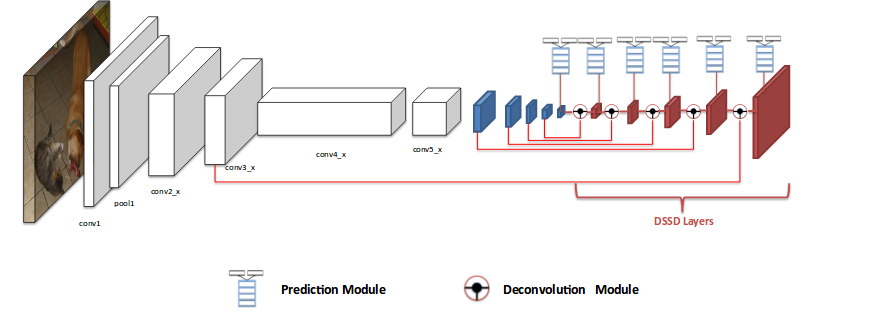
\includegraphics[scale=0.4]{./tex/computer-vision/sota/dssd.png}
\caption{Architecture de Deconvolutional Single Shot Detector (DSSD)}
\label{dssd}
\end{figure}

\begin{figure}
\centering
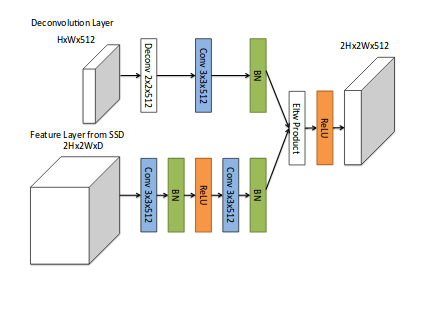
\includegraphics[scale=0.4]{./tex/computer-vision/sota/deconvmod.png}
\caption{Architecture du Deconvolution module de DSSD}
\label{deconvmodfig}
\end{figure}

\begin{figure}
\centering
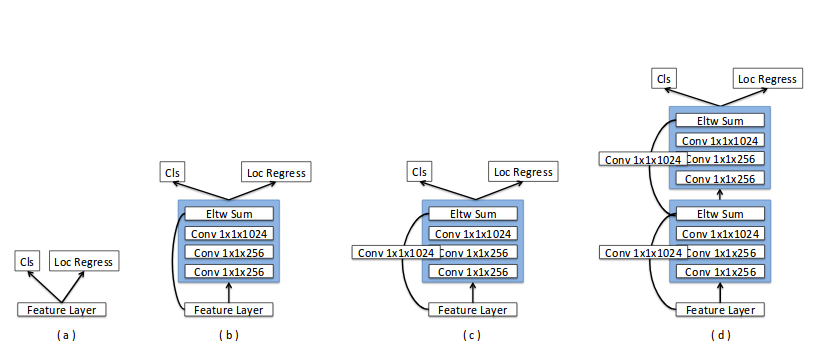
\includegraphics[scale=0.4]{./tex/computer-vision/sota/predmoddssd.png}
\caption{Architecture du module prédictif de DSSD}
\label{predmoddssd}
\end{figure}

\subsubsection{RetinaNet}
Une des contraintes principales des modèles d'\textit{Object Detection} est la différence de distribution entre les classifications positives et négatives du fait du nombre très importants de \textit{bounding boxes} proposées pour chaque image. Deux approches sont exploitées aujourd'hui: exploiter une sous-parties des données prédites afin d'exploiter une distribution avantageuses (\textit{Hard Negative Mining} par exemple) ou appliquer une pondération spécifique dans la fonction de coût. Le modèle \textit{RetinaNet}\cite{retinanet} exploite la seconde approche en proposant une nouvelle fonction de perte: \textit{Focal Loss}.

\paragraph{Focal Loss}
\textit{Focal Loss} est une nouvelle fonction de perte basée sur \textit{Cross-Entropy}. Son approche propose de pondérer la valeur de l'erreur produite en fonction des probabilités issues des prédictions afin de favoriser l'expression des erreurs de prédiction. En effet, \textit{Cross-Entropy} impose une erreur (même faible) pour toute prédiction non parfaite, i.e différente de la valeur de la données d'apprentissage (souvent 1 pour la classe correspondante). Cette imperfection du modèle n'a pas d'influence sur la performance du modèle. En effet, la prédiction reste inchangée que la probabilité soit de 1 ou de 0.7 par exemple. Cependant, pour la fonction de perte, cette différence est majeure car les vraies erreurs sont noyées par l'effet de bord produit par les bonnes prédictions "imparfaites". Afin de pondérer les vraies erreurs du modèle, \textit{Focal Loss} propose une pondération de l'erreur selon sa probabilité prédite. Elle est définie par:
$$p_t=\left\{ \begin{array}{ll} p \  \  \  \  \  \  \  \  \  \  \  if \ y_{classe,ref}=1\\ 1-p \  \  \  \  \  \ otherwise \end{array} \right. $$
$$FL(p_t)=-\alpha(1-p_t)^\gamma log(p_t)$$
\noindent Avec $\alpha$ et $\gamma$, hyperparamètres du modèle. En supposant $\gamma=2$ et $\alpha=1$, si $p_t=0.9$ alors son erreur sera 100x plus faible que l'erreur produite par \textit{Cross-Entropy} par exemple. Cette réduction permet de s'émanciper du déséquilibre entre les distributions de classes et d'éviter l'étape de \textit{sampling} consistant à ramener le minibatch d'apprentissage à un ratio 3:1. Le comportement de \textit{Focal Loss} est visible sur la Figure \ref{focallosscurve}. Pour $\gamma=0$, \textit{Focal Loss} est identique à \textit{Cross-Entropy}. Expérimentalement, les créateurs du modèle ont observé que les meilleurs résultats expérimentaux sont obtenus avec $\gamma=2$. Avec cette configuration, on peut observer que l'erreur pour les probabilités supérieures à 0.6 est quasi-nulle. Néanmoins, cette approche pénalise la confiance du modèle pour ne considérer que la prédiction finale. Ainsi, d'un point de vue métier, le modèle favorise les bonnes prédictions au détriment de la confiance en ses prédictions. Par conséquent, bien qu'il y ait une amélioration de prédiction empiriquement, les résultats sont moins fiables. Il peut donc être délicat d'employer ce genre de métrique lorsque l'on recherche un résultat avec une forte probabilité de certitude.

\begin{figure}
\centering
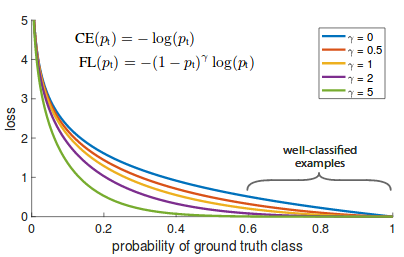
\includegraphics[scale=0.4]{./tex/computer-vision/sota/focallosspic.png}
\caption{Erreur obtenue par Focal Loss selon $\gamma$}
\label{focallosscurve}
\end{figure}

\paragraph{Le modèle RetinaNet}
L'architecture de \textit{RetinaNet} ne présente pas de nouveautés notables et repose sur des architectures connues. Ainsi, \textit{RetinaNet} exploite une architecture \textit{Resnet} pour l'extraction d'attributs associée à un \textit{Feature Pyramid Network}\footnote{Voir Section \ref{fepyramide} pour plus de détails} (FPN) pour extraires les \textit{feature map} de prédiction. L'approche \textit{Anchor boxes} est utilisée pour définir les \textit{bounding boxes}. La classification et la détermination des coordonnées de la \textit{bounding boxes} sont définies par deux réseaux \textit{Full Convolutionnal Network} indépendants, i.e ils ne partagent pas les mêmes paramètres. Une illustration de l'architecture de \textit{RetinaNet} est visible sur la Figure \ref{retinanetfig}.\\

\noindent L'utilisation de procédés ayant démontrés leurs efficacités associée à une fonction de perte plus performante que les modèles précédents font de \textit{RetinaNet}, l'un voire le modèle le plus performant actuellement. Seule sa vitesse de prédiction est préjudiciable, faisant de YOLO la seule alternative véritablement convaincante selon les circonstances.

\begin{figure}
\centering
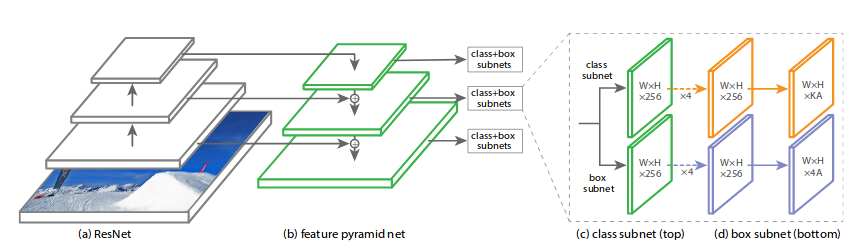
\includegraphics[scale=0.4]{./tex/computer-vision/sota/retinanetpic.png}
\caption{Architecture du réseau RetinaNet}
\label{retinanetfig}
\end{figure}

\subsubsection{Comparatif des modèles récents}
Sur la Figure \ref{compobj1}, nous pouvons observer un comparatif sur le jeu de données COCO selon la métrique mAP. Comment on peut le constater, les modèles \textit{Retina} sont les plus performants que ce soit en temps de prédiction ou de précision. Seul YOLO est significativement plus rapide en contrepartie d'une précision moindre. Il est important de comprendre que ce comparatif est réalisé selon un mAP strict. Il n'est pas toujours pertinent d'avoir une prédiction avec une précision très importante. En effet, d'un point de vue métier, il n'est pas forcément utile d'être au pixel-près.\\

\noindent Sur la Figure \ref{compobj2}, le même comparatif est réalisé avec un mAP placé à 0.5\footnote{C'est une métrique standard pour les compétitions de modèles}. L'exigence de précision est donc plus faible mais reste suffisamment stricte pour garantir une exploitation métier satisfaisante. On observe que YOLOv3 devient significativement meilleur que précédemment. Sa vitesse d'exécution est significativement plus rapide que les autres modèles et ce, pour une qualité de prédiction meilleure ou équivalente. Seule FPN FRCN est plus précis en contrepartie d'un temps de prédiction nettement plus important. \\

\noindent On peut donc conclure que \textit{Retina} est le choix de référence pour la précision du modèle lorsqu'une forte exigence est requise. Au contraire, lorsque l'exigence est moindre, YOLOv3 offre un compromis vitesse/précision remarquable et FPN FRCN, la meilleure précision malgré un temps de calculs élevé.

\begin{figure}
\centering
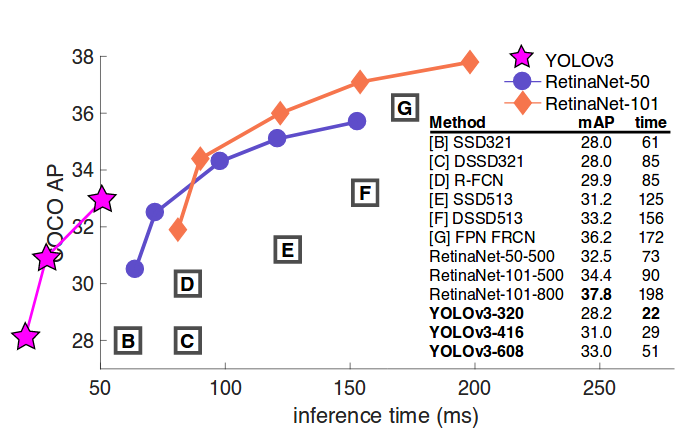
\includegraphics[scale=0.4]{./tex/computer-vision/sota/comp3.png}
\caption{Comparatif des modèles d'Object Detection}
\label{compobj1}
\end{figure}

\begin{figure}
\centering
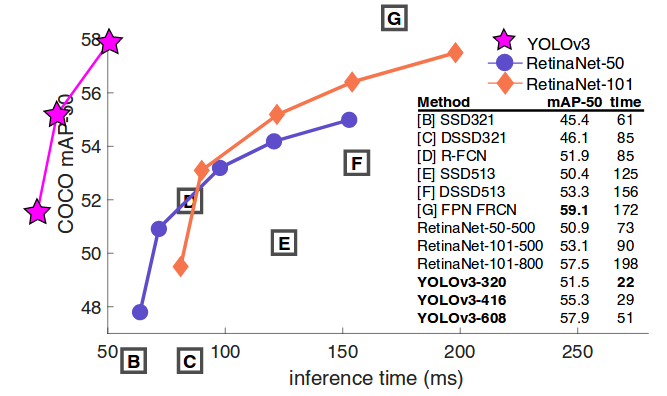
\includegraphics[scale=0.4]{./tex/computer-vision/sota/comp4.png}
\caption{Comparatif des modèles d'Object Detection pour un mAP à 0.5 IoU}
\label{compobj2}
\end{figure}
